\documentclass[a4paper 12pt]{article}
\usepackage[margin=1in]{geometry}
\usepackage{natbib}
\usepackage{epsfig}
\usepackage{amsmath}
\usepackage{amsfonts}
\usepackage{float}
\usepackage{rotating} 
\usepackage{caption}
\usepackage{subfig}
\usepackage{booktabs}
\usepackage{adjustbox}
\usepackage[table]{xcolor}
\usepackage{tabularx}
\usepackage{caption}
\usepackage{enumerate}
\usepackage{enumitem}
\captionsetup{font=footnotesize}
\newcommand{\ra}[1]{\renewcommand{\arraystretch}{#1}}
\textheight 9.0 in
\textwidth 6.5 in
\topmargin -0.5 in
\oddsidemargin 0.0in
\renewcommand{\topfraction}{1}
\renewcommand{\bottomfraction}{1}
\renewcommand{\textfraction}{0}
\renewcommand{\floatpagefraction}{0.90}
\definecolor{TableEven}{rgb}{0.8000,0.9216,0.9490}
\usepackage{makecell}
%\usepackage{fourier} 
\numberwithin{equation}{section}
\usepackage{array}
\usepackage{titlesec}
\usepackage{sectsty}
\sectionfont{\centering}
\setcounter{secnumdepth}{4}
\usepackage{natbib}
\usepackage{siunitx}
\usepackage[toc,page]{appendix}
\usepackage{sectsty}
\usepackage{scalerel,stackengine}
\stackMath
\usepackage{graphicx}
%\titleformat{\subsection}    
%       {\normalfont\fontfamily{phv}\fontsize{12}{17}\bfseries\itshape}{\thesubsection}{1em}{}
\subsectionfont{\normalfont\bfseries\itshape}
\subsubsectionfont{\normalfont\itshape}
%\usepackage[colorlinks,citecolor=DeepPink4,linkcolor=DarkRed, urlcolor=DarkBlue]{hyperref}
%\usepackage[svgnames]{xcolor} 
%
%\usepackage[colorlinks]{hyperref}
%\hypersetup{citecolor=DeepPink4}
%\hypersetup{linkcolor=DarkRed}
%\hypersetup{urlcolor=DarkBlue}
%\usepackage{cleveref}

%hyperlink for website will need a better option. highlights all equations etc
 \usepackage{hyperref}


\renewcommand{\baselinestretch} {2.0}
\makeatletter
\setcounter{page}{1}
\def\doublespace{\def\baselinestretch{1}\@normalsize}
\def\enddoublespace{}
\title{\bf 
}   
% \footnotemark}
\author{}
\date{}
\@addtoreset{equation}{section}
\renewcommand{\sp}{\vspace{0.2 in}}
\renewcommand{\theequation} {\arabic{section}.\arabic{equation}}
%\renewcommand{\thefigure}{\arabic{section}.\arabic{figure}}
\renewcommand{\thefootnote}{\fnsymbol{footnote}}
\newtheorem{theorem}{Theorem}
\newtheorem{lemma}{Lemma}[section]
\newtheorem{remark}{Remark}[section]
\newtheorem{corollary}{Corollary}[section]
\newtheorem{exam}{Example}[section]
\newtheorem{proposition}{Proposition}[section]

\newcommand{\Bigskip}{\vspace{0.3 in}}

\usepackage{xspace}
\newcommand{\m}{\textnormal{\sffamily m}\xspace}
\newcommand{\cm}{\textnormal{\sffamily cm}\xspace}
\newcommand{\g}{\textnormal{\sffamily g}\xspace}
\newcommand{\kg}{\textnormal{\sffamily kg}\xspace}
\newcommand{\SE}{\textnormal{\sffamily SE}\xspace}
\newcommand{\RSE}{\textnormal{\sffamily RSE}\xspace}
\newcommand{\LB}{\textnormal{\sffamily LB}\xspace}
\newcommand{\UB}{\textnormal{\sffamily UB}\xspace}


\makeatletter
\let\latex@xfloat=\@xfloat
\def\@xfloat #1[#2]{%
  \latex@xfloat #1[#2]%
  \def\baselinestretch{1}
  \@normalsize\normalsize
  \normalsize
}
\makeatother

\newcommand\longitude[1]{\directlua{ longitude ( \luastring{#1} ) }}


\usepackage{lineno}
\linenumbers

 
\begin{document}
\title{An analysis of the North Sea International Bottom Trawl Survey Data}

\maketitle


\begin{abstract}
In this research we present non-parametric estimation procedures for calculating abundance at age indices, and investigate the sensitivity of these estimates with respect to the number of otholits collected at sea. The procedures presented are applied to the North Sea International Bottom Trawls Survey data for cod (\textit{Gadus morhua}) and saithe (\textit{Pollachius virens}). We demonstrate how much information would be lost if the survey design was defined such that fewer otholits were collected. Age length keys (ALKs) are used to map lengths to age, and we use ALKs with and without the assumption of constant age length structures over relatively large areas. All abundance at age indices are presented with variance estimates. \\

%Currently, such variance estimates are \textit{only} utilized for assessment of Herring (\textit{Clupea harengus}) in the North Sea, even thou they may include valuable information from the survey. \\

%{\bf The abundance at age indices introduced differ from non-parametric indices provided by IBTS by how the age given length relation (ALK) is included}.  We use ALK's without the assumption of constant ALK over pre-defined areas\\

%age length keys are used to map lengths to age, and we use ALKs with and without the assumption of constant age length structures over relatively large areas (over predefined areas)

%The North Sea International Bottom Trawl Survey (IBTS) was started by the International Centre for the  Exploration of the Sea (ICES) in 1990. Seven research vessels using standardized fishing methods participates in the survey. The survey with these vessels, which allows fishing also on rough ground provides information on seasonal distribution of stocks and abundance,  which forms the basis for stock assessments. Estimates of abundance indices based on age-length keys (ALK) are provided without any assessment of their accuracy.  We present a model-based ALK estimator, and a stratified design-based ALK estimator for estimating abundance at age. Both estimators take into the spatial differences in age-length structures. These estimators are compared with the designed-based ALK estimator proposed by ICES for IBTS, which does not account for spatial differences in the age-length structure. As the proposed ALK estimator by ICES is a combination of age data over a large area, this can result in biased estimates of numbers-at-age. An example of cod (\emph{Gadus morhua}) in ICES subareas IVa and IVb is used to illustrate spatial differences in the proportions of age-at-length, and estimates of uncertainty are presented using nonparametric bootstrapping. In general, the model-based ALK estimator provides a more accurate coverage probabilities compared with the other estimators.  
\end{abstract}


\section{Introduction}
Fish stock assessments are used by fishery managers for making management decisions regarding catch quotas. The assessments provide fundamental information about the status of the stock, for instance, whether the stock is increasing and support for increased levels of harvest should be given, or whether the stock is decreasing and stricter control on harvest should be implemented. Associated with the parameters used in fish stock assessment is their uncertainty, which should not be ignored when formulating management policies \citep{walters1981effects, ludwig1981measurement, berg2014evaluation}. This uncertainty can arise from many sources including natural variability, estimation procedures and lack of knowledge regarding the parameter \citep{ehrhardt1997role}. The North Sea International Bottom Trawl Survey (IBTS) data, coordinated by the International Council for the Exploration of the Sea (ICES), provides information on seasonal distribution of stocks and estimates of abundance indices and catch in numbers of fish per age-class without an assessment of the accuracy of these estimates. As stated by \citet{ludwig1981measurement} it is relevant for managers to take into the uncertainty related to stock size when making management polices. The indices of abundance at age from IBTS  are based on data obtained from a stratified semi-random sampling approach of trawl stations,  and  it is essential to account for the sampling approach so as to produce reliable variance estimates \citep{lehtonen2004practical}. If the sampling approach is ignored, the effect on the variance  of the parameters could be substantial.  In particular, the variance could be greatly inflated  due to the clustering effect, which involves intra-cluster correlation of the variables \citep{aanes2015efficient, lehtonen2004practical}. 

There are two separate stages of the North Sea International Bottom Trawl Survey (IBTS) for generating abundance indices per age.  The first consist of calculating indices per \textit{length} class, which are obtained by trawling in a stratified manner and counting the number of fish caught. Then that knowledge is transformed to indices with respect to age. The latter part is achieved with an age-length key (ALK), which is constructed by sampling otoliths in a stratified procedure from each haul and/or sub-area. To our best knowledge, there has been no research on how much the uncertainty of the abundance indices is related to these two distinct parts. The main contribution of this article is to shed light on how the indices estimates and their associated uncertainty estimates change if less effort was spent on collection of otoliths. We achieve the reduction of otoliths by mimicking a defined sampling procedure with less effort. We also focus on the spatial distribution of the ALK, and such spatial structures in the ALK has also been investigated in \citet{berg2012spatial, hirst2012bayesian}.

Currently, abundance indices from IBTS are reported in DATRAS \citep{datras} using an age-length key (ALK) \citep{fridriksson1934calculation} which is assumed to be constant over relatively large areas. In this research we propose two ALKs which accounts for spatial variation: i) a nonparametric  haul based ALK, and ii) a spatial model-based ALK. These ALKs are described in section \ref{sec:methods}, and the results from the model based ALK gives a strong case for assuming variation in the ALK within RFAs. %In section \ref{sec:modelBasedALK} we introduce a spatial model based ALK, and see figure \ref{fig:40cmCod2015} for an illustration of spatial variation in the ALK. 
A spatial model based ALK \citep{berg2012spatial, berg2014evaluation} known as the NS-IBTS Delta-GAM index \citep{ICES2016b} is currently being used to calculate standardized age-based survey indices used in assessment for the North Sea stock. And as far as we are aware the variance estimates of parameters estimated from NS-IBTS Delta-GAM index  are \textit{only} utilized for assessment of Herring (\textit{Clupea harengus}) in the North Sea.
%even thou they may include valuable information from the survey.} \\

The spatial ALK model introduced in \citet{berg2012spatial} is similar to the model used in this paper; the main difference is that we include the spatial structure through a spatial random field \citep{lindgren2011explicit} and not through two dimensional splines \citep{wood2017generalized}.%(see Figure \ref{fig:40cmCod2015}, which shows the estimated age probabilities of a 40 cm cod (\emph{Gadhus morhua}) in the first quarter of 2015). Figure \ref{fig:40cmCod2015} shows that the age distribution clearly varies for a 40 cm cod within Central North Sea and Northern North Sea (see second graph in the first panel). 
 An  overview of the  North Sea International Bottom Trawl Survey is given in Section \ref{overview}. The current estimators for ALK and catch per unit effort (CPUE) used by ICES in their database for trawl surveys (DATRAS) and our proposed ALK estimators are given in Section \ref{sec:methods}. Two case studies, in which the methods described in Section \ref{sec:methods} are applied to, are given in Section \ref{sec:data}, and a discussion is given in Section \ref{sec:discussion}.% The results are given in Section \ref{sec:results} and a discussion is given in Section \ref{sec:discussion}.



\subsection{Overview of the North Sea International Bottom Trawl Survey}
\label{overview}
\indent The North Sea International Bottom Trawl Survey was formed in 1991, which is a combination of the International Young Herring Survey (IYHS) and eight national surveys in the North Sea, Skagerrak and Kattegat areas. These surveys began in the 1960's, and the 1970's and 1980's, respectively. The IYHS was developed with the aim of obtaining annual recruitment indices for the combined North Sea herring \emph{Clupea harengus} stock \citep{ICES2012}, but yielded valuable information on other fish species such as cod \emph{Gadus morhua} and haddock \emph{Melanogrammus aeglefinus}.\\
\indent The North Sea IBTS began with quarterly surveys providing information on seasonal distribution of stocks sampled, hydrography and the environment, which allows changes in fish stock to be monitored and abundance of all fish species to be determined. These quarterly surveys, however became difficult to sustain as countries experienced budget cuts making it impossible to maintain high levels of research vessel effort. As such, in 1997 countries carried out a survey only twice a year; a first quarter survey (January-February) and a third quarter survey (August-September). The target species of IBTS fished from 1991-2018 includes standard pelagic species: Herring (Clupea harengus), Sprat (Sprattus sprattus) and Mackerel (Scomber scombrus); and standard roundfish species: Cod (Gadus morhua), Haddock (Melanogrammus aeglefinus), Saithe (Pollachius virens),  Norway Pout (Trisopterus esmarkii)  and Whiting (Merlangius merlangus).

% Table \ref{fishspecies} gives the common names (scientific names in parentheses) of the target species that are sampled during the quarterly North Sea International Bottom Trawl Surveys. The common names of the species in parentheses will be used in the rest of paper.\\
%\clearpage
%\begin{small}
%\begin{table}[h!]
%\centering
%\setlength\tabcolsep{1.5pt} 
%\captionsetup{font=small, width = 8.5cm}{
%\caption{Species fished in the NS-IBTS from 1991-2017.}\label{fishspecies}}
%\begin{tabular}{cccccccccc}
%\hline \\
%\multicolumn{2}{c}{} \\
%Standard Pelagic               & Standard Roundfish & By-Catch Gadoid       \\[1.5ex]
%\hline \\[0.1ex]
%Herring (Clupea harengus) &  Cod (Gadus morhua)  & Pollock (Pollachius)      \\[1.5ex]
%Sprat (Sprattus sprattus)   &Haddock (Melanogrammus aeglefinus) & Pouting (Trisopterus luscus) \\[1.5ex]
%Mackerel (Scomber scombrus) & Norway Pout (Trisopterus esmarkii) & Trisopterus minutus (Poor Cod) \\[1.5ex]
% & Saithe (Pollachius virens)  & Blue Whiting (Micromesistius poutassou)   \\[1.5ex]
%&Whiting (Merlangius merlangus)  & Hake (Merluccius merluccius)  \\[1.5ex]
%& &  Ling (Molva molva) \\[1.5ex]
%& &  Tusk (Brosme brosme) \\[0.5ex]
%\hline
%\end{tabular}
%\end{table}
%\end{small}
Research vessels from seven nations in the first quarter (Q1) and six nations in the third quarter (Q3) are used for conducting surveys on all finfish species in the North Sea during January-February and July-August, respectively, between 1997-2018 (Table \ref{countries} in Web appendix \ref{secAp:areasfishedappendix} gives details of the different research vessels). The sampling frame is defined by the ICES index or roundfish areas (RFA) as shown in Figure \ref{icesroufismap} numbered 1 to 10, and which we refer to as superstrata \citep{nottestad2015quantifying, fuller2011sampling}. These  roundfish areas were substratified into small strata defined by non-overlapping statistical rectangles of roughly $30 \times 30$ nautical miles ($1^{o} \  \mathrm{Longitude} \ \times  \  0.5^{o} \ \mathrm{Latitude}$), and were convenient to use for North Sea IBTS as they were already being used for fisheries management purposes. Most statistical rectangles contain a number of possible tows that are deemed free of obstructions, and vessels are free to choose any position in the rectangles as long as the hauls are separated by at least 10 nautical miles within and between rectangles. However, all countries select tows based on a semi-random approach from datababes of national safe tows or DATRAS or commercial fishing data, except Sweden who uses fixed stations and in some cases depth-stratified semi-random sampling design \citep{ICES2018}, and England who also uses fixed stations and only conduct surveys during the third quarter. In some rectangles, sampling may be further stratified due to significant changes in seabed depth which may, in turn, cause variations in the fish population. In particular, the North Sea IBTS herring, saithe and sprat data are weighted by depth strata in the statistical rectangle (see Table \ref{tab:weights} in appendix \ref{secAp:weightings}). It is also a requirement that countries avoid clustering their stations between adjacent rectangles in order to reduce positive serial correlation, and thereby maximize survey precision.  The latest major reallocation of rectangles occurred in 1991, but since then the survey has tried to keep at least one vessel in every subarea in which it had fished in the most recent years. Minor reallocation of rectangles between Norway, Scotland and Germany was done in 2013. Each rectangle was  typically sampled twice by two different countries before 1997, but after that target coverage of two trawl hauls per rectangle per survey  was introduced because of national financial constraints \citep{ICES2015}. But in some rectangles in the Eastern English Channel, Southern North Sea and Central North Sea intensified sampling is carried out.\\
\indent The recommended standard trawling gear of the North Sea IBTS is the mulitpurpose chalut {\`a} Grande Ouverture Verticale (GOV) trawl \citep{ICES2012}, which has been used on all participating vessels since 1992, while different pelagic and bottom trawls suitable for fishing finfish species were used before 1992. Standardized trawling protocols were adopted with a towing speed of 4 knots but depending on vessel performance, tide and weather conditions the average towing speed can be at minimum 3.5 and maximum 4.5 knots. From 2000-2018 trawling is done during the daylight hours, which are considered 15 minutes before sunrise to 15 minutes  after sunset \citep{ICES2012}. After each trawl the total catch of the different species is weighed on board and biological parameters such as length for all fish species caught (to 0.1$\cm$ below for shellfish, to 0.5$\cm$ below for herring and sprat and to 1$\cm$ below for all other species) are collected. Where the numbers of individuals are too large for all of them  to be measured to obtain the length distribution, a representative subsample of 100 fish is selected. Otoliths are collected on board from a small fraction of all the target species from all RFAs (Figure \ref{icesroufismap}) to retrieve age reading. Table \ref{tab:otolithsTable} in Web appendix \ref{secAp:otolithappendix} gives the minimum sampling levels of otoliths for the target species.
%\indent The trawl tow locations are selected using a  semi-random approach with at least two primary sampling units (PSU) per stratum, where PSUs are standardized swept-area trawl hauls. Sampling locations for all countries are proposed in advance in order to increase the randomisation of sampling. These locations are based on a random selection on a random selection of valid tows with start and end position executed in the period 2000-2017. In the unusual event that no ``clear" tow exists the cruise leader, who select the haul positions, may select to undertake a ``blind" tow on unknown ground after checking the proposed trawl track for hazardous seadbed obstructions with acoustic methods. \\
%\clearpage
%\begin{figure}[h!]
%  \centering
% {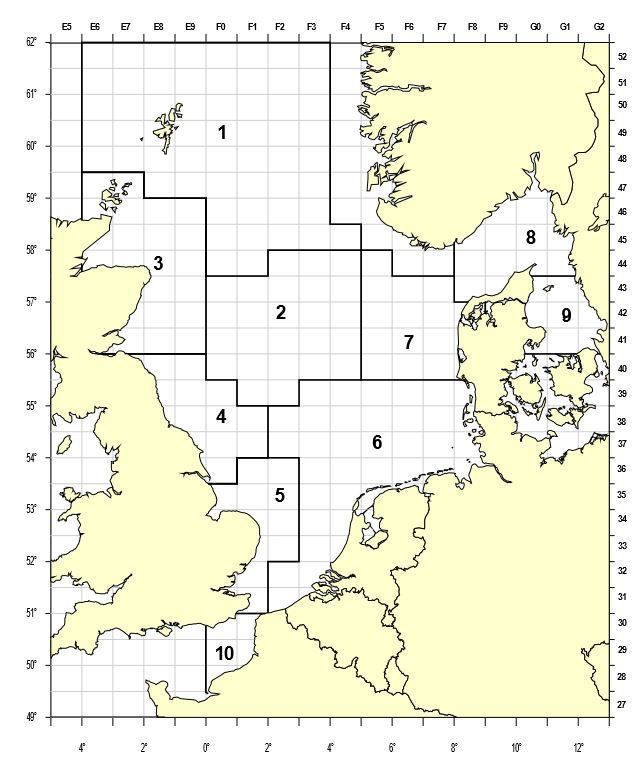
\includegraphics[width=8.5cm]{icesroundfishmap.jpg}}   
% \captionsetup{font= footnotesize, width=13cm}{
% \caption{Standard roundfish areas used for roundfish since 1980, for all standard species since 1991. Additional RFA 10 added in 2009. For example, the number 1 indicates ICES Index Area 1, and an ICES Statitical rectangle (ST) in IA 1 is 43F1 \citep{ICES2015}.}\label{icesroufismap}}
%\end{figure}

%\clearpage
\begin{figure*}[h!]
\centering
\begin{tabular}{@{}ccc@{}}
\subfloat[]{\includegraphics[width=1.0\textwidth]{surveyarea}} & 
%\subfloat[Map of IBTS Q3]{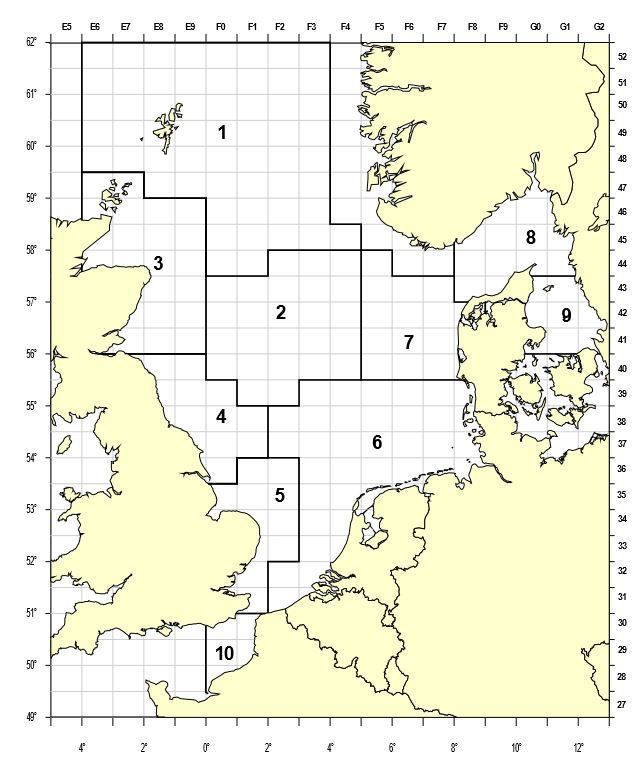
\includegraphics[width=0.45\textwidth]{icesroundfishmap.jpg}} &
\end{tabular}
\caption[]{Standard roundfish areas used for roundfish since 1980, for all standard species since 1991 (left panel). Additional RFA 10 added in 2009. For example, the number 1 indicates ICES Index Area 1, and an ICES Statitical rectangle (ST) in IA 1 is 43F1. The map on the right panel shows norwegian trench and shelf edge (depths 1000-1500).}
\label{icesroufismap}
\end{figure*} 



\section{\large METHODS}
\label{sec:methods}
This section gives the estimators of abundance indices. The estimators are haul time-based and utilizes an ALK approach. We consider the ALK approach used in DATRAS and we propose two ALK estimators. The ALK used in DATRAS for computing abundance indices does not account explicitly for the spatial distribution in the age-length composition, which may be different and would result in a biased ALK. This difference may be caused either by variation in length-at-age distributions or by variations in the relative abundance of age classes, that is age-at-length distributions \citep{gerritsen2006simple}.  To account for the spatial distribution we propose a design-based ALK estimator that is haul dependent (Section \ref{sec:haulestimator}) and a model-based ALK estimator (\ref{sec:spatialModelALK}).
\subsection{Catch per unit effort}
\label{sec:cpueestimators}
In this research, the catch per unit effort (CPUE) is defined as the number of fish of a certain species and age or length which are caught per hour trawl. In this section we define the CPUE mathematically, which explains how the index is calculated. 

For a given species of interest, let $n_{h,l}$ be the number of fish with length $l$ caught by trawl haul $h$. The CPUE for a given length $l$ by trawl haul $h$ is defined as 
\begin{equation}\label{eq:cpueHaul}
\mathrm{CPUE}_{h,l} =\frac{n_{h,l}}{d_h},
\end{equation}
were $d_h$ is the duration of the trawl in hours. The CPUE per age class is further defined as
\begin{equation}\label{eq:cpueALK}
\mathrm{CPUE}_{h,a} =\sum_{l \in {\bf L}}\mathrm{CPUE}_{h, l} \times ALK_{a,l,h},
\end{equation}
where ${\bf L}$ is the set of all length classes and $ALK_{a,l,h}$ is the age length key, which represents the estimated proportion of fish with age $a$ in $l$th length class in haul $h$. For a given number of trawl hauls in a statistical rectangle, the mean CPUE defined as  mCPUE  in a statistical rectangle can be expressed as the average CPUE of the trawl hauls in the statistical rectangle:
\begin{equation}\label{eq:cpueRec}
\mathrm{mCPUE}_{s,a} =\sum_{h \in H_{s}}\frac{\mathrm{CPUE}_{h,a}}{|H_{s}|}.
\end{equation}
Here $H_{s}$ represents the set of trawl hauls taken in statistical rectangle $s$, and $|H_{s}|$ is the number of hauls taken in the rectangle. The mCPUE in $p$th RFA is further defined as
\begin{equation}\label{eq:cpueRFA}
\mathrm{mCPUE}_{p,a} = \sum_{s \in S_{p}} \frac{\mathrm{mCPUE}_{s,a}}{|S_{p}|} \omega_s,
\end{equation}
where $S_{p}$ is the set of all statistical rectangles in RFA $p$, $|S_{p}|$ is the number of statistical rectangles in RFA $p$, and $\omega_s$ is a weight variable for each statistical rectangle. The weight variable $\omega_s$ varies between species. For some species $\omega$ equals 1 (e.g. Gadus morhua) for all $s$, and for other species it is the proportion of the statistical rectangle which has depth between 10 to 200 meters, for example Pollachius virens (see Table \ref{tab:weights} in Web appendix \ref{secAp:weightings}  for weightings of statistical rectangles).  The index for abundance at age in the whole study area, $\lambda_{a}$, is further defined by
\begin{equation}
\lambda_{a}= \frac{\sum_{p\in {\bf P}} A_{p}  \mathrm{mCPUE}_{p,a}}{A_{\text{total}}}.
\label{abundanceestimatornorthsea}
\end{equation}
Here ${\bf P}$ is the set of RFAs, $A_p$ is the area of RFA $p$, and $A_{\text{total}} = \sum_{p\in {\bf P}} A_{p}$.
%mCPUE_{N,a} 
 

\subsection{ALK estimators}
\label{sec:alkmethods}

The definition of the CPUE of age includes an ALK, see (\ref{eq:cpueALK}), which we described in this section. Three ALK estimators are included in this research, which are named as follows:  \textit{i}) DATRAS ALK, \textit{ii}) haul based ALK and \textit{iii}) model based ALK.
% In this section we define these three ALK estimators. 
\subsubsection{DATRAS ALK}
\label{sec:datrasalkestimator}
Let $\text{ALK}^{\text{D}}$ denote the DATRAS ALK. The $\text{ALK}^{\text{D}}$ is defined as constant within each RFA, and is calculated for each RFA by aggregating the age observation from each RFA. $ALK^{\text{D}}_{a,l,h}$ used in equation (\ref{eq:cpueALK}) is defined as the proportion of observed fish with age $a$ in length class $l$ in the RFA $h$. If there are no observed fish in length class $l$ in the RFA, ages from length classes close to $l$ is used. The details of the procedure for borrowing strength from neighbouring length classes are given in Web appendix \ref{secAp:DATRASBorrow}. The underlying assumption of this ALK  is that age-length compositions are homogeneous within the RFAs. This is a rather strong assumption, and any violation would have an unknown impact on the estimates of abundance indices. \citet{aanes2015efficient} illustrated that violation of the assumption of constant ALK leads to biased estimates of CPUEs. 

\subsubsection{Haul based ALK}
\label{sec:haulestimator}
We define a haul dependent ALK  by  $ALK^{H}$. The $ALK^{H}_{a,l,h}$ is defined as the average proportion of observed fish with age $a$ in  length class $l$ in haul $h$. If there are no observed ages of fish in a length class $l$ in the haul, ages from the same length class in the haul close by is used (Web appendix \ref{secAp:oursBorrow} describes the procedure in detail).

\subsubsection{Spatial model-based ALK estimator}
\label{sec:spatialModelALK}
In this section we introduce a spatial model based ALK. Using such a model enables us to obtain smooth structures in the distribution of age given length. It further enables us to utilize spatial latent effects. Spatial model-based approach of age-lengths are widely used \citep{berg2012spatial, hirst2012bayesian, rindorf2001analyses}, and are used for stock assessment in the North Sea \citep{berg2014evaluation}. \\ % kvist2000using olav: double check this when i have access.
\indent Let the response variable of the age group of a fish be $a = M,...,A$ where $M$ is the youngest age, and $A$ is the oldest age which is typically defined as a "plus group". Suppose $y(l,{\bf s},h)$ is the age  of a fish with length $l$ caught at location ${\bf s}$. As in \citet{berg2012spatial} we use a continuous ratio model for the spatial age given length model. Define
\begin{align}\label{eq:linearPred1}
\pi_a[y(l,{\bf s})] = P(y = a|y \geq a, l, {\bf s}) = \frac{p_a(l,{\bf s})}{p_a(l,{\bf s}) + \cdots p_{A-1}(l,{\bf s})} \vspace{ 4mm} \ \ \ \text{for } a =M,...,A-1 ,
\end{align}
where $p_a(l,s)$ is the probability of a fish with length $l$ at location ${\bf s}$ to be of age $a$. Note that $\pi_a(y(l,{\bf s}))$ is the probability of age $a$ given that it has age greater than or equal to its age with length $l$ at location $s$. Further is it assumed a logit link
\begin{align}\label{eq:linearPred}
\log \left[ \frac{\pi_a[y(l,{\bf s})]}{1-\pi_a[y(l,{\bf s})]}\right] = \beta_a +  f_a(l) + \gamma_a({\bf s}).
\end{align}
Here $\beta_a$ is an intercept, $ f_a(l)$ is a continuous function of length and $\pmb{\gamma}$ is a mean zero Gaussian spatial random field with Mat\'{e}rn covariance function. The spatial random field is intended to capture any spatial variation in the ALK.

The continuous function $f_a(l)$ in (\ref{eq:linearPred}) is modelled with usage of P-splines \citep{wood2017generalized}, and these spline regression coefficients are included as a Gaussian random effect. The precision matrix for the spline regression coefficients is constructed such that the variability (or wryggliness) in the spline is penalized, see \citet[page 239]{wood2017generalized} for details. The R package mgcv \citep{wood2015package} is used for extracting the precision matrix needed for the spline regression coefficients.

\indent We assume that the spatially Gaussian random field in (\ref{eq:linearPred}), $\pmb{\gamma}$, follows a stationary Mat\'{e}rn covariance structure:
\begin{equation}\label{eq:matern}
 \text{Cov}(\gamma(\mathbf{s}_1),\gamma(\mathbf{s}_2)) = \frac{\sigma^2_{\gamma}}{2^{\nu-1}\Gamma(\nu)}(\kappa_{\gamma}||\mathbf{s}_1 -\mathbf{s}_2||)^{\nu}K_{\nu}(\kappa_{\gamma}||\mathbf{s}_1-\mathbf{s}_2||),
\end{equation}
where $\sigma^2_{\gamma}$ is the marginal variance, $||\cdot||$ is the Euclidean distance measure in kilometres, $\nu$ is a smoothing parameter, $\kappa_{\gamma}$ is a spatial scale parameter and $K_{\nu}(\cdot)$ is the modified Bessel function of the second kind with $\nu = 1$. The spatial field is estimated with the stochastic partial differential equation (SPDE) procedure described in \citet{lindgren2011explicit}. The main concept behind the SPDE procedure is that the precision matrix of a spatial field with Mat\'{e}rn  covariance function can be approximated by a sparse matrix on a grid covering the area of interest. Such a grid and sparse precision matrix are constructed with use of the R-INLA package \citep{rue2009approximate}.

The model based ALK estimate is obtained by maximizing the likelihood. We maximize the likelihood with use of an R-Package called Template Model Building {\sffamily TMB} \citep{kristensen2015tmb}, combined with the optimizing function {\sffamily nlminb} in R. In this application {\sffamily TMB} is advantageous as it uses Laplace approximation for the latent fields gaining computational efficiency, it also utilizes sparse structures in the latent fields, and uses automatic derivation. 


\subsection{Uncertainty estimation}
\label{sec:uncertaintyestimation}
In this section we describe how the uncertainty of the CPUE estimates are calculated. We use nonparametric bootstrapping to quantify the uncertainty of the CPUEs. In nonparametric bootstrapping independent samples of lengths and age are drawn with replacement from the original data and approximate $95\%$ confidence intervals are obtained using bias-corrected percentile method  \citep{carpenter2000bootstrap}. Nonparametric resampling allows us to estimate the sampling distribution of the CPUE empirically without making assumptions concerning the data. The bias-Corrected method adjusts for the bias and skew of the sampling distribution of the data. This method assumes that there is a montonic increasing function and the estimator $\hat{\lambda}_{a}$ has a monotonic increasing function $f()$ such that the transformed values $f(\hat{\lambda}_{a})$ are normally distributed with mean $f(\rho) - z_{0}$ and standard deviation one, where $z_{0}$ are the standard normal limits \citep{puth2015variety}.

A bootstrap procedure for estimating the uncertainty of CPUEs in the North Sea is suggested in  \citet{ICES2013}. In the rest of this research, we refer to this procedure as DATRAS bootstrap procedure. The DATRAS procedure is divided into two parts; one part which samples CPUE per length (\ref{eq:cpueHaul}), and another part which samples the ALK used in (\ref{eq:cpueALK}). The DATRAS bootstrap procedure is based on the assumption of homogeneous CPUE within RFAs. This assumption is likely to be wrong, and will typically cause an overestimation of the uncertainty.  Therefore, we have included a bootstrap procedure, defined as the stratified bootstrap procedure, which instead assumes constant CPUE within each statistical rectangle. 

\subsubsection{DATRAS and Stratified bootstrap procedure}
\label{sec:datrasstratifiedbootstrap}
In this section we describe the bootstrap procedure for catch at length proposed by \emph{DATRAS} \citep{ICES2013} and the stratified procedure, and elaborate how the ALK is simulated. Assume there are $N_{\text{s}}$ trawl hauls in a statistical rectangle. The DATRAS bootstrap procedure consists of sampling with replacement $N_{\text{s}}$ of all trawl hauls in the corresponding RFA, and place them in the statistical rectangle. This procedure is performed independently across all statistical rectangles. It should be remembered that this procedure is based on the assumption that ALK is homogeneous in the whole RFA, and the implication of DATRAS bootstrap procedure on indices of abundance is two-fold. Firstly, DATRAS bootstrap procedure ignores the fine-scale stratification in the sampling process. This would lead to an overestimation of the uncertainty. Secondly, it ignores the sampling procedure of age-length data collected at the haul level. This would lead  to an underestimation of the uncertainty. So there are biases in both directions, which are difficult to quantify.

The Stratified bootstrap procedure is a modification of the DATRAS bootstrap procedure. Rather than sampling hauls from the whole RFA, we  sample the $N_{\text{s}}$ trawl hauls from the list of hauls within the same statistical rectangle. If there is only one trawl haul within a statistical rectangle, we sample either that haul or the closest haul.

For simulating the DATRAS ALK we sample with replacement age observations within each RFA stratified with respect to length. If there is only one observed age from a given length class, we sample either that age or, at random, an age of the closest length class with observed ages. For the haul based ALK, we use the observed ages in the sampled hauls when simulating the CPUE per length ({\bf is this from the stratified bootstrap procedure? what about explanations for the model based ALK? We also have codes for stratified procedure where DATRAS ALK is used, should we mention that this is done INSTEAD or AS WELL and include this results below in results section? Jon Helge mentioned that it's not plausible to show results of DATRAS bootstrap as it does not account for the survey design. Better off using our proposed stratified procedure with DATRAS ALK; include results for DATRAS using their suggested bootstrap procedure in appendix and reference in paper concerning higher variances}).

\subsection{Reducing sampling effort}
\label{sec:optimizationsampling}

The current sampling procedure for the North Sea IBTS data is the sampling of one otolith from every observed length group in every trawl (see Table \ref{tab:otolithsTable} in Web appendix \ref{secAp:otolithappendix}). We investigate the effect on the estimated mCPUE and its variance if the sampling procedure of otoliths changes such that fewer otoliths were collected. To determine this effect we remove otholits in a stratified manner, mimicking a sampling procedure where fewer otoliths are collected. For sampling fewer otoliths, we define wider length groups, for example $2$ cm, or $3$ cm, or $5$ cm and so on,  and simulate the otolith  collection such that only one otolith is sampled from every wider length group. Estimated mCPUE's with summary statistics, based on the simulated reduced data sets are then compared with the parameters estimated from using all of data. In principle, we are free to define any length class to reduce the number of observed otoliths. For simplicity we propose two procedures: i) sample at random  one otolith from every 2 cm length group, and ii) sample at random one otolith from every 5 cm length group. 


\section{Case studies}
\label{sec:data}
In this section we apply the methods described in Section \ref{sec:methods} to data from the International Bottom Trawl Survey for the years 2017-2018, which is obtained from the DATRAS database \citep{datras}. These years are chosen for two reasons. The first is that in year 2018 new sampling procedures proposed by ICES for the collection of otoliths were introduced in the surveys. For instance, one otolith per length group is sampled for most target species (see Table \ref{tab:otolithsTable} in Web appendix \ref{secAp:otolithappendix} for details of the sampling procedures for each target species), and this data is appropriate for the application of our proposed sample optimization procedure described in Section \ref{sec:optimizationsampling}. The second is that IBTS included Age 0 in Q3 surveys, and since data for year 2018 Q3 is not yet available, the data for years 2017 Q3 and 2018 Q1 will be used in our analyses. Also, some species such as saithe that occupies the deeper waters in the northern part of the North Sea and in the Skagerrak and Kattegat, along the shelf edge \citep{ICESFishMaps}, the IBTS Q3 data is relevant for analyses compared with data from IBTS Q1 surveys, which do not adequately cover these areas where saithe is distributed (see Figure \ref{icesroufismap}). Note that both IBTS Q1 and Q3 surveys do not adequately cover the whole stock distribution of saithe but the data collected is considered generally representative \citep{ICESJune2016}.

In this research, the species of interest are cod and saithe. All samples are caught using the standard GOV gear described in Section \ref{overview}. Table \ref{tab:data2018} gives a brief description of the data for year 2018 in the first quarter and year 2017 in the third quarter.  Cod can be as old as 12 years in the first quarter and 11 years in the third quarter; and saithe as old as 18 years in the first quarter and 17 years in the third quarter. In our analyses we consider the age groups 1 to 6+ in Q1 and 0 to 6+ in Q3 for all ALK methods, where the last group consists of fish of age 6 or older. Saithe are typically older than cod but smaller in length, particularly in Q1. Catch rates are higher in the third quarter, 48\% for cod and 164\% for saithe, compared with the first quarter.\\
%the IBTS Q3 surveys  cover wider areas in the north sea. 

\clearpage
\begin{small}
\begin{table}[h!]
\caption{Summary of North Sea IBTS cod and saithe (in parentheses) data for third quarter in year 2017 and first quarter in year 2018.}
\begin{tabular}{llllll}
\toprule
\bf Data&\bf Description \\
\midrule
Trawl hauls  & Total of 372 trawl hauls in year 2018 Q1; 238 (83)  with length and 230 (81) \\ & with age information. In 2017 Q3, a total of 349 trawl hauls were taken; \\ & 238 (129) with length and 237 (128) with age information. \\[1.7ex]

Age &The age varied between 1 (1) to 12 (18) years in year 2018 Q1 and \\ & 0 (0) to 11 (17) in year 2017 Q3. \\[1.7ex]

Length & Length information in cm varied between 11 (13) to 114 (106) cm in year 2018 Q1 \\ & and between 6 (10) to 112 (109) cm in year 2017 Q3. \\[1.7ex]

Date&Date of catch in year 2018 Q1 varied between 15.01.2018 to 28.02.2018 \\ & and in year 2017 Q3 between 18.07.2017 to 31.08.2018 \\[1.7ex]

Duration of haul & Mean duration is 29.37 minutes, with 30 minutes as 83\% coverage interval \\ & in year 2018 Q1; and in 2017 Q3 with mean duration of 29.26 minutes \\ & with 30 minutes as 88\% coverage . \\[1.7ex]

Total count for all ages & 1511 (793) in year 2018 Q1 and 2236 (2092) 2017 Q3. \\[0.5ex]
\bottomrule
\end{tabular}
\label{tab:data2018}
\end{table}
\end{small}


\subsection{Estimated indices of abundance and variability for cod and saithe}
\label{sec:codresults}

In this section we apply the three ALK methods given in section \ref{sec:alkmethods} for abundance estimation, and the bias-corrected bootstrap method, given in Section \ref{sec:datrasstratifiedbootstrap} for estimating variability of estimated indices of abundance. 

Recall that the main assumption of DATRAS ALK is that the age-length compositions of species over large areas are the same. To illustrate that this assumption may not be valid, we used  the spatial ALK model (\ref{eq:linearPred}) to predict probabilities of age given length of a 40 cm long cod and a 40 cm long saithe in the North Sea (Figure \ref{predictedprobabilitiesplot}). These plots provide strong evidence against a null hypothesis of no spatial effect in the ALKs, as the likelihood of age given length changes in some areas. Figure \ref{predictedprobabilitiesplot} (a) shows that the eastern North Sea in RFAs 7 and 8 (the regions in yellow) is one of the areas where a 40 cm cod is more likely to be age 3. A saithe of 40 cm is more likely to be 3 years or older.The plots also show that cod is distributed in all areas of the North Sea, except RFA 10 (Figure \ref{predictedprobabilitiesplot} (a)), whereas saithe is more likely to inhabit deeper areas in the northern North Sea, specifically RFA 1, and Skagerrak in  RFA 8 (Figure \ref{predictedprobabilitiesplot} (b) and Figure \ref{icesroufismap}, right panel). 

%{\bf plot probability graph for saithe}

\clearpage
\begin{figure}[h!]
\centering
\begin{minipage}[c]{1.10\linewidth}
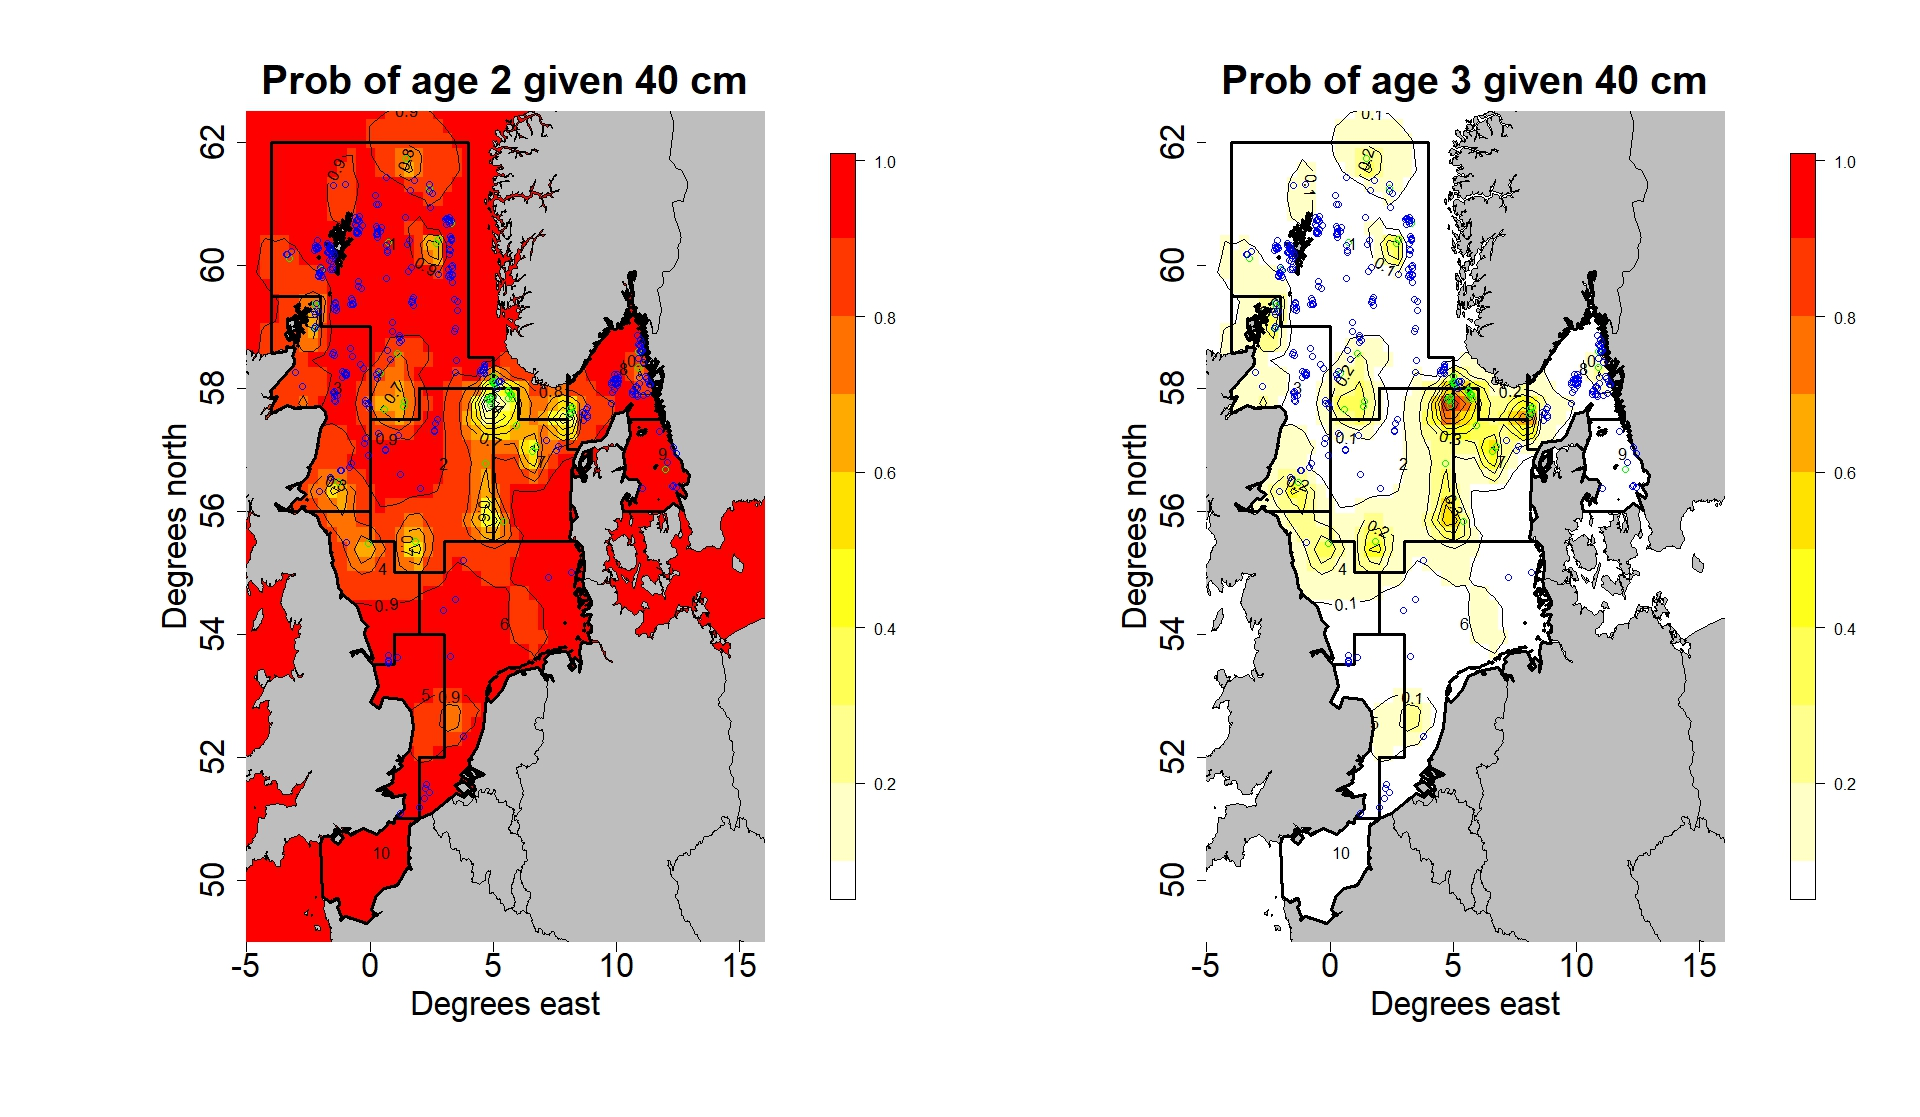
\includegraphics[width=170mm,scale=6.5]{cod2018Q1Map.jpeg}
\caption*{ (a) Probability plot of 40 cm cod in year 2018 Q1.}
\label{fig1.1}
\end{minipage}

\quad
\begin{minipage}[c]{1.10\linewidth}
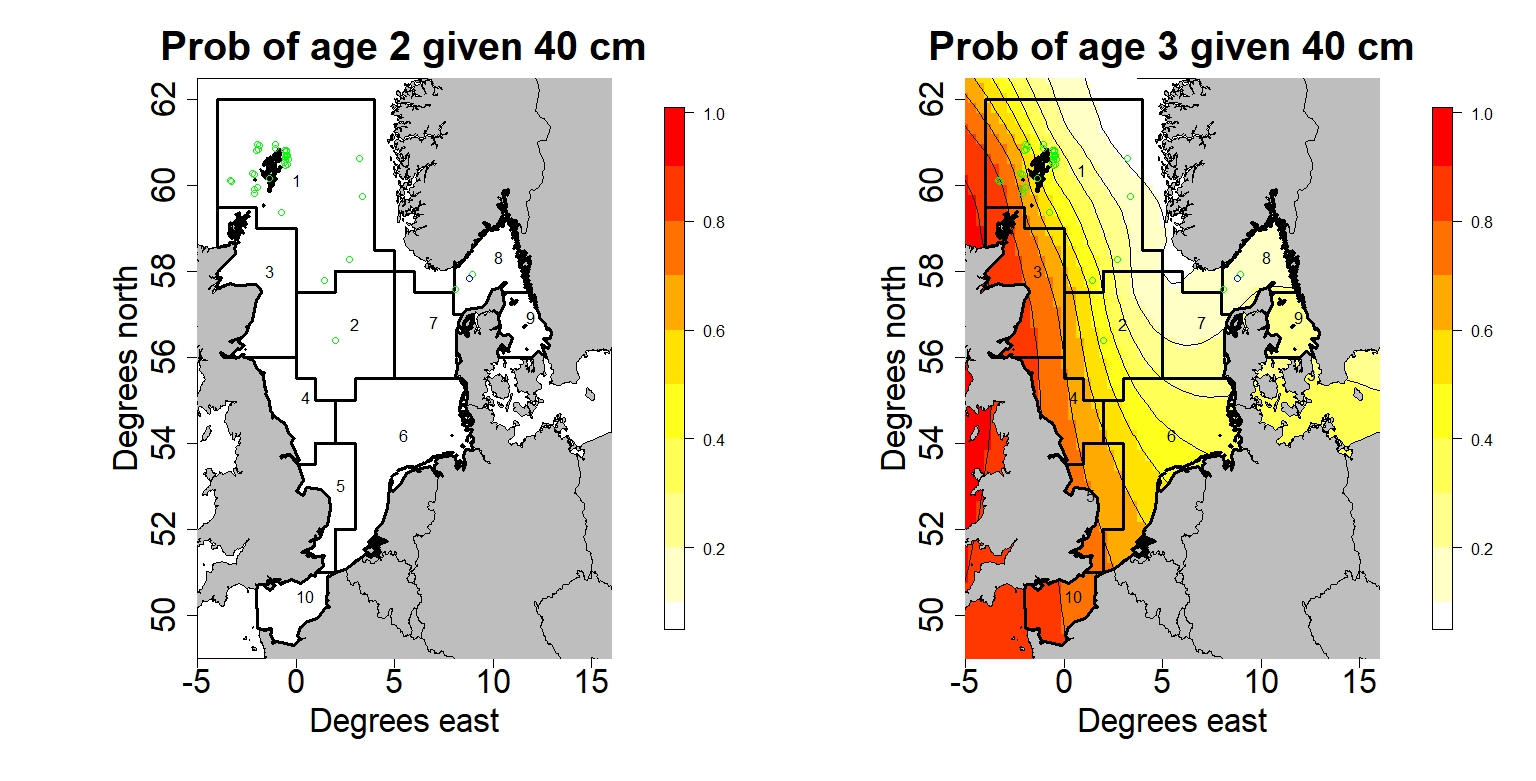
\includegraphics[width=170mm,scale=6.5]{saithe2018Q1Map.jpeg}
\caption*{(b) Probability plot of 40 cm saithe in year 2018 Q1}
\label{fig5.1}
\end{minipage}
\captionsetup{font=small, width = 14.5cm}{
 \caption{Predicted probabilities of age given length using model (\ref{eq:linearPred1}) and (\ref{eq:linearPred}) for the year 2018 Q1. Graph (a) gives probabilities of predicted age of a 40 cm long cod, and graph (b) gives probabilities of predicted age of a 40 cm saithe in RFAs 1 to 10 in the North Sea. The small coloured circles ($\circ$, blue or green) are the trawl hauls with cod or saithe data.}\label{predictedprobabilitiesplot}}
\end{figure}


\clearpage
Figures \ref{percentileBiascorrectedCIcod} and  \ref{percentileBiascorrectedCIsaithe} give estimates of indices of abundance for cod in years 2017 Q3 and 2018 Q1, and  saithe in year 2017 Q3. Approximate 95\% confidence intervals from the bias-corrected bootstrap method for 200 bootstrap replication are estimated from the three ALK methods. The stratified procedure described in \ref{sec:datrasstratifiedbootstrap} is used in the sampling process to estimate bootstrap confidence intervals.   

Figures \ref{percentileBiascorrectedCIcod} and  \ref{percentileBiascorrectedCIsaithe} show that the resulting indices of abundance turned out to be similar for all ALKs. However, the implication of not accounting for variability over wider areas is higher  uncertainty in the estimates, as shown by the the percentage relative standard error (RSE\%) from DATRAS ALK. 


%We would expect higher uncertainty estimates for older fishes from our ALK methods compared with DATRAS as variability is much higher for this group due to small sample sizes. However, in Q3 for both species estimated uncertainty is from our ALKs is similar or smaller compared with DATRAS ALK for the plus group......\\

{\bf Discuss model base ALK results here....problems with variance-covariance structure etc using the required number of linear predictors e.g. A-1 or A-2 or an alternative approach to the fisher information or Hessian matrix, such as bootstrapping, for uncertainty estimation}\\



For illustration we show the implications of using DATRAS bootstrap procedure for estimating the uncertainty around indices of abundance  in Figure \ref{percentileBiascorrectedCIProcedures} in Web appendix \ref{secAp:resultsdatrasALK}. Compared with the stratified bootstrap procedure, DATRAS bootstrap procedure gives an overestimation of the uncertainty for all age groups, suggesting that it is highly relevant to account for the variation in the data over large areas ({\bf need to generate this plot for appendix}). 

{\bf re-run codes with updated ALK model for cod and saithe in 2017 Q3 plots}


\clearpage

\begin{figure*}[h!]
\centering
\begin{tabular}{@{}ccc@{}}
\subfloat[Cod in year 2018 Q1]{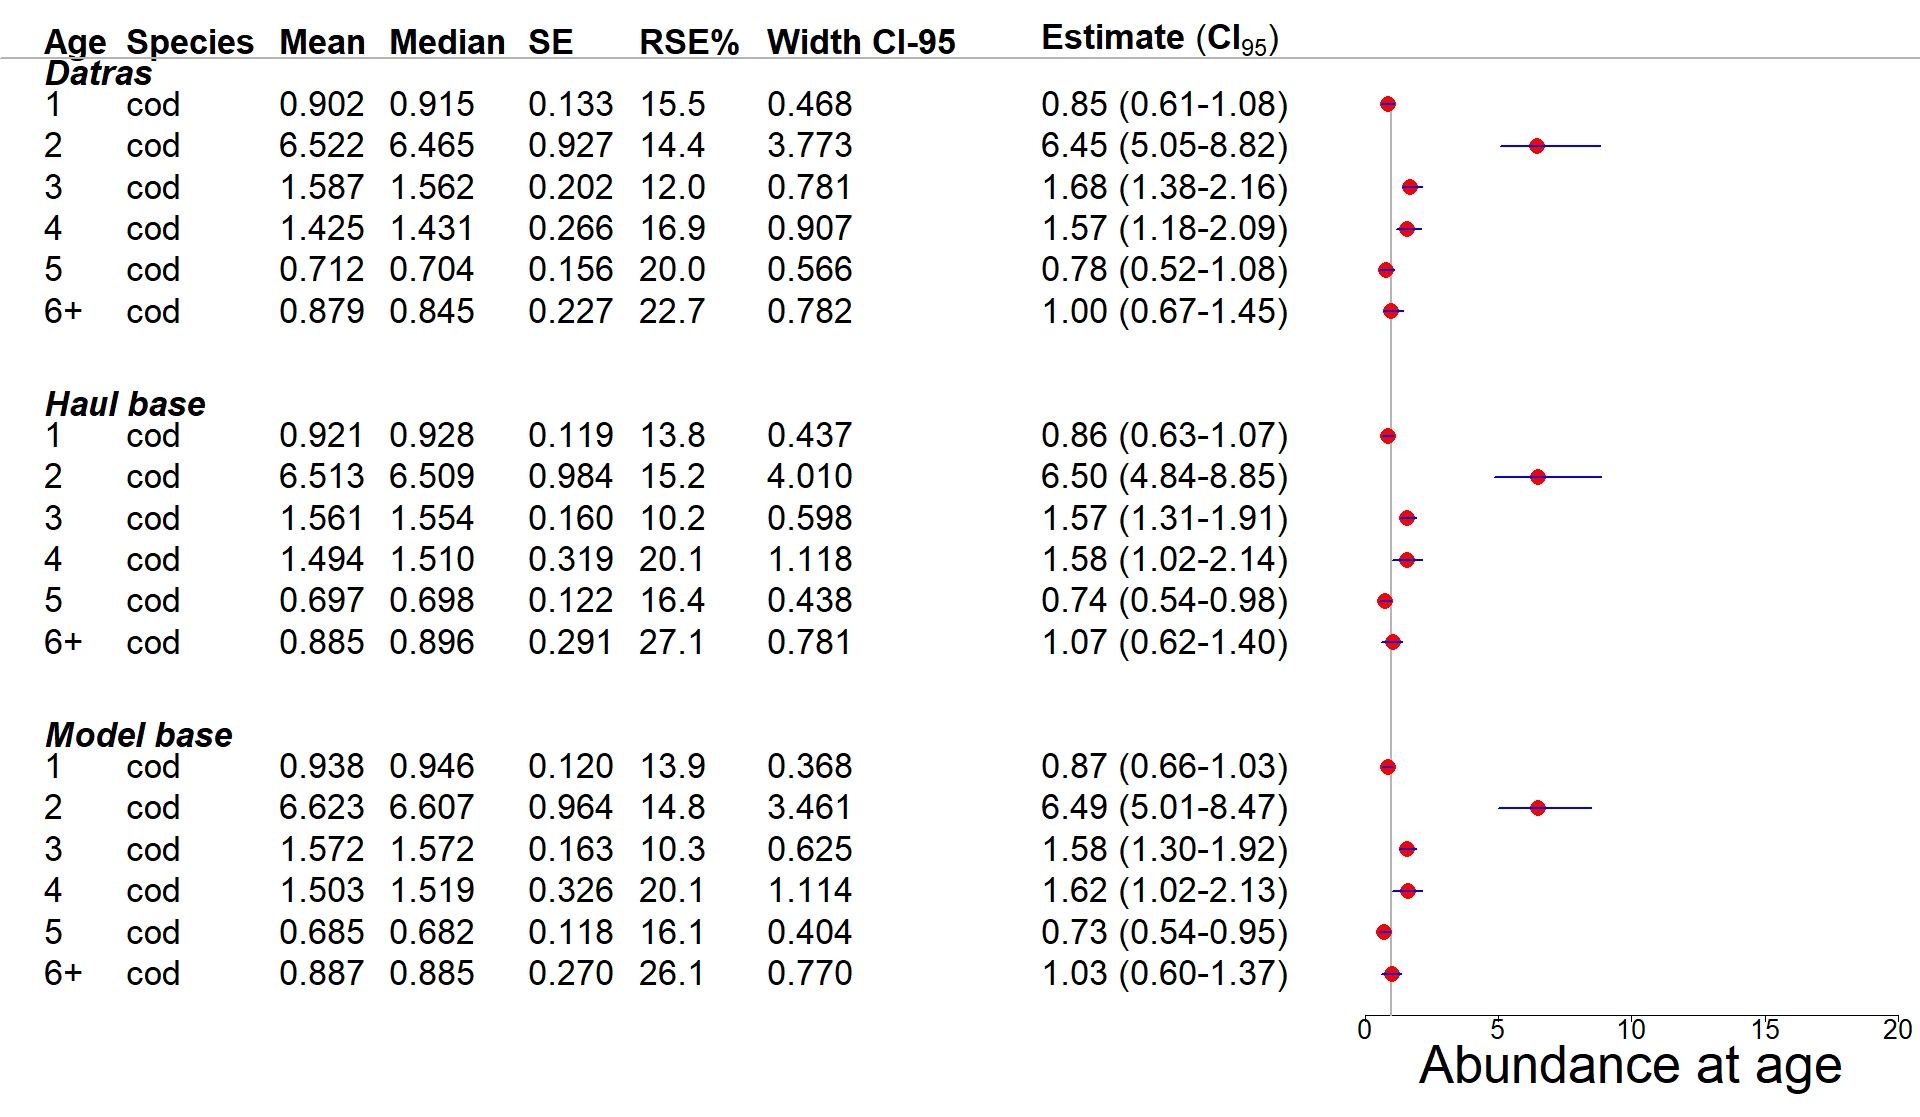
\includegraphics[width=0.95\textwidth]{cod2018Q1BiasCorr.jpeg}} & \\
\subfloat[Cod in year 2017 Q3]{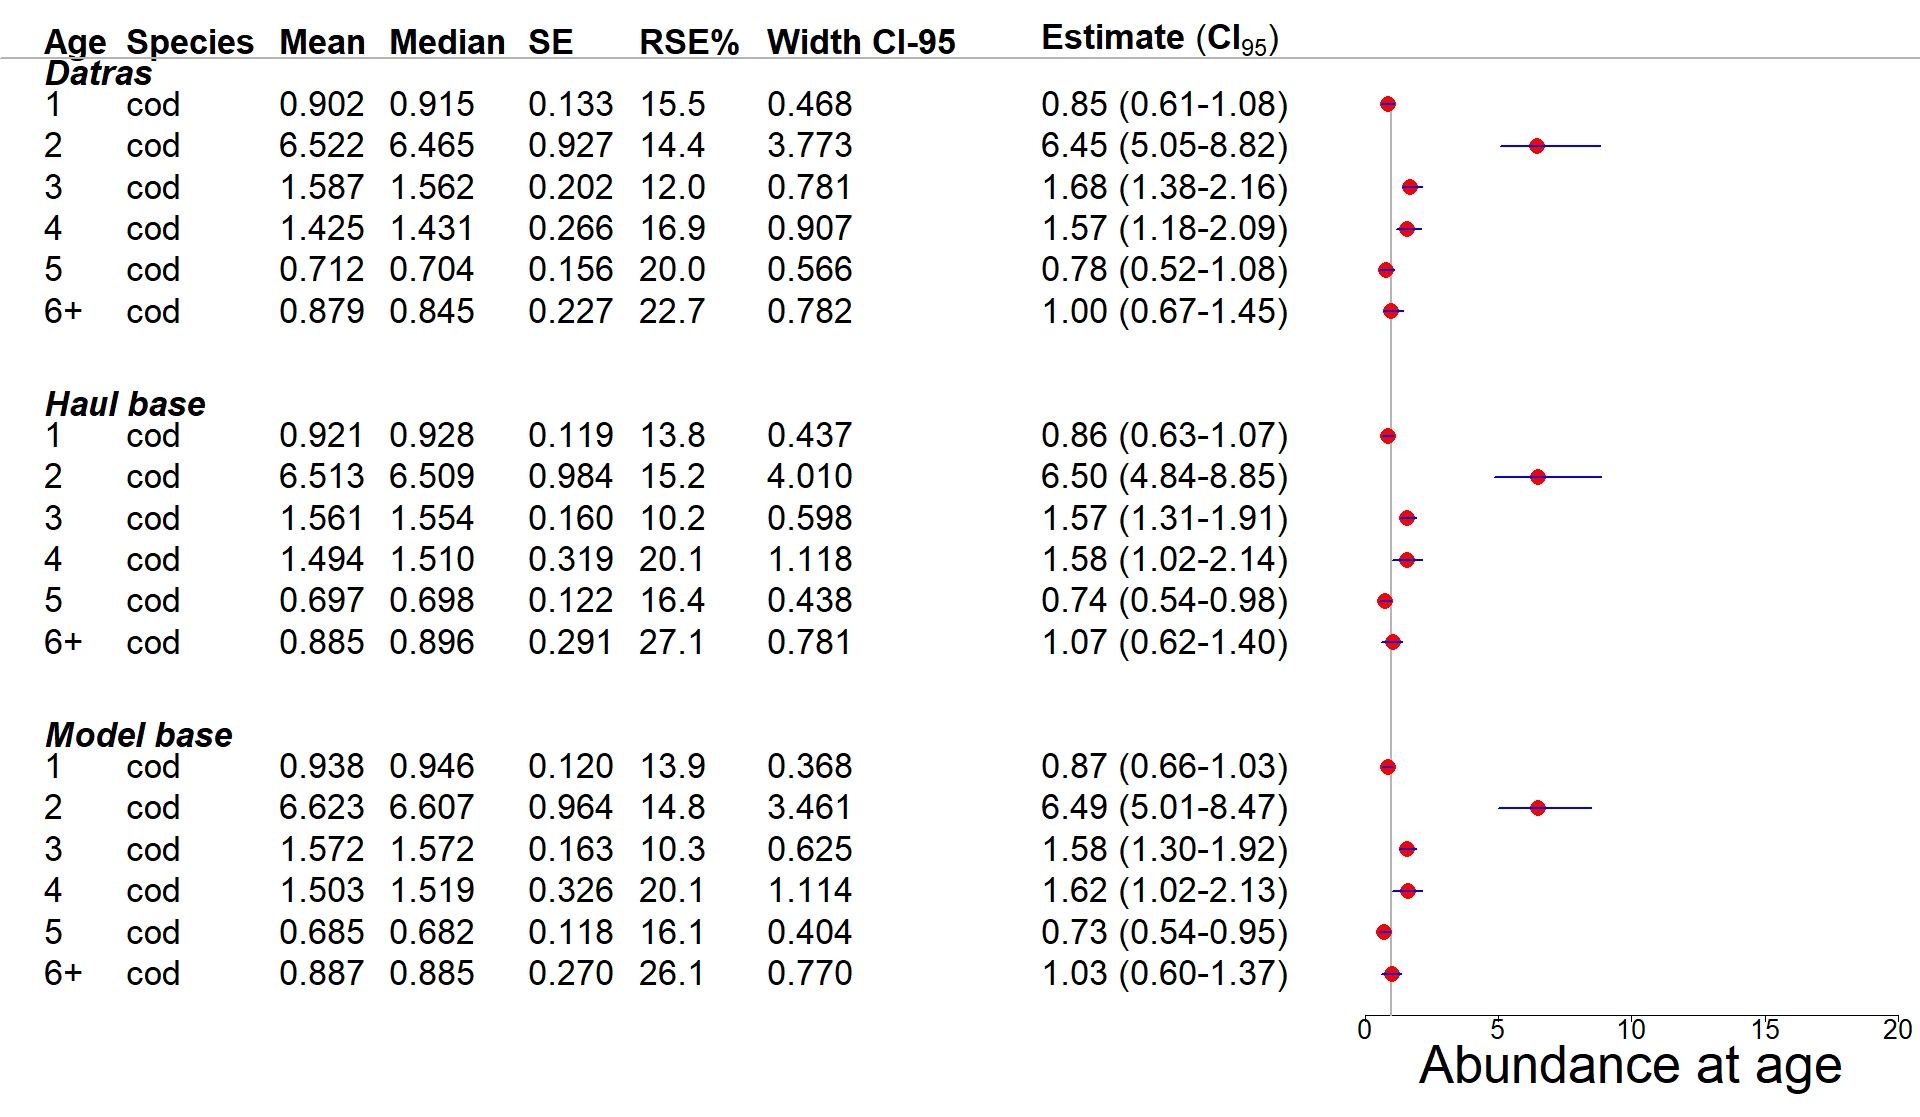
\includegraphics[width=0.95\textwidth]{cod2018Q1BiasCorr.jpeg}} &
\end{tabular}
\caption[]{Estimated confidence intervals ($\mathrm{CI}_{95}$) from bias-corrected  bootstrap method for cod in years 2017 Q3 and 2018 Q1. Estimated indices of abundance (Estimate), and its standard error (SE), percentage relative standard error (RSE\%), and bootstrap mean (mean)  and median estimates are also given.}
\label{percentileBiascorrectedCIcod}
\end{figure*} 

\clearpage

\begin{figure*}[h!]
\centering
\begin{tabular}{@{}ccc@{}}
\subfloat[Saithe in year 2018 Q1]{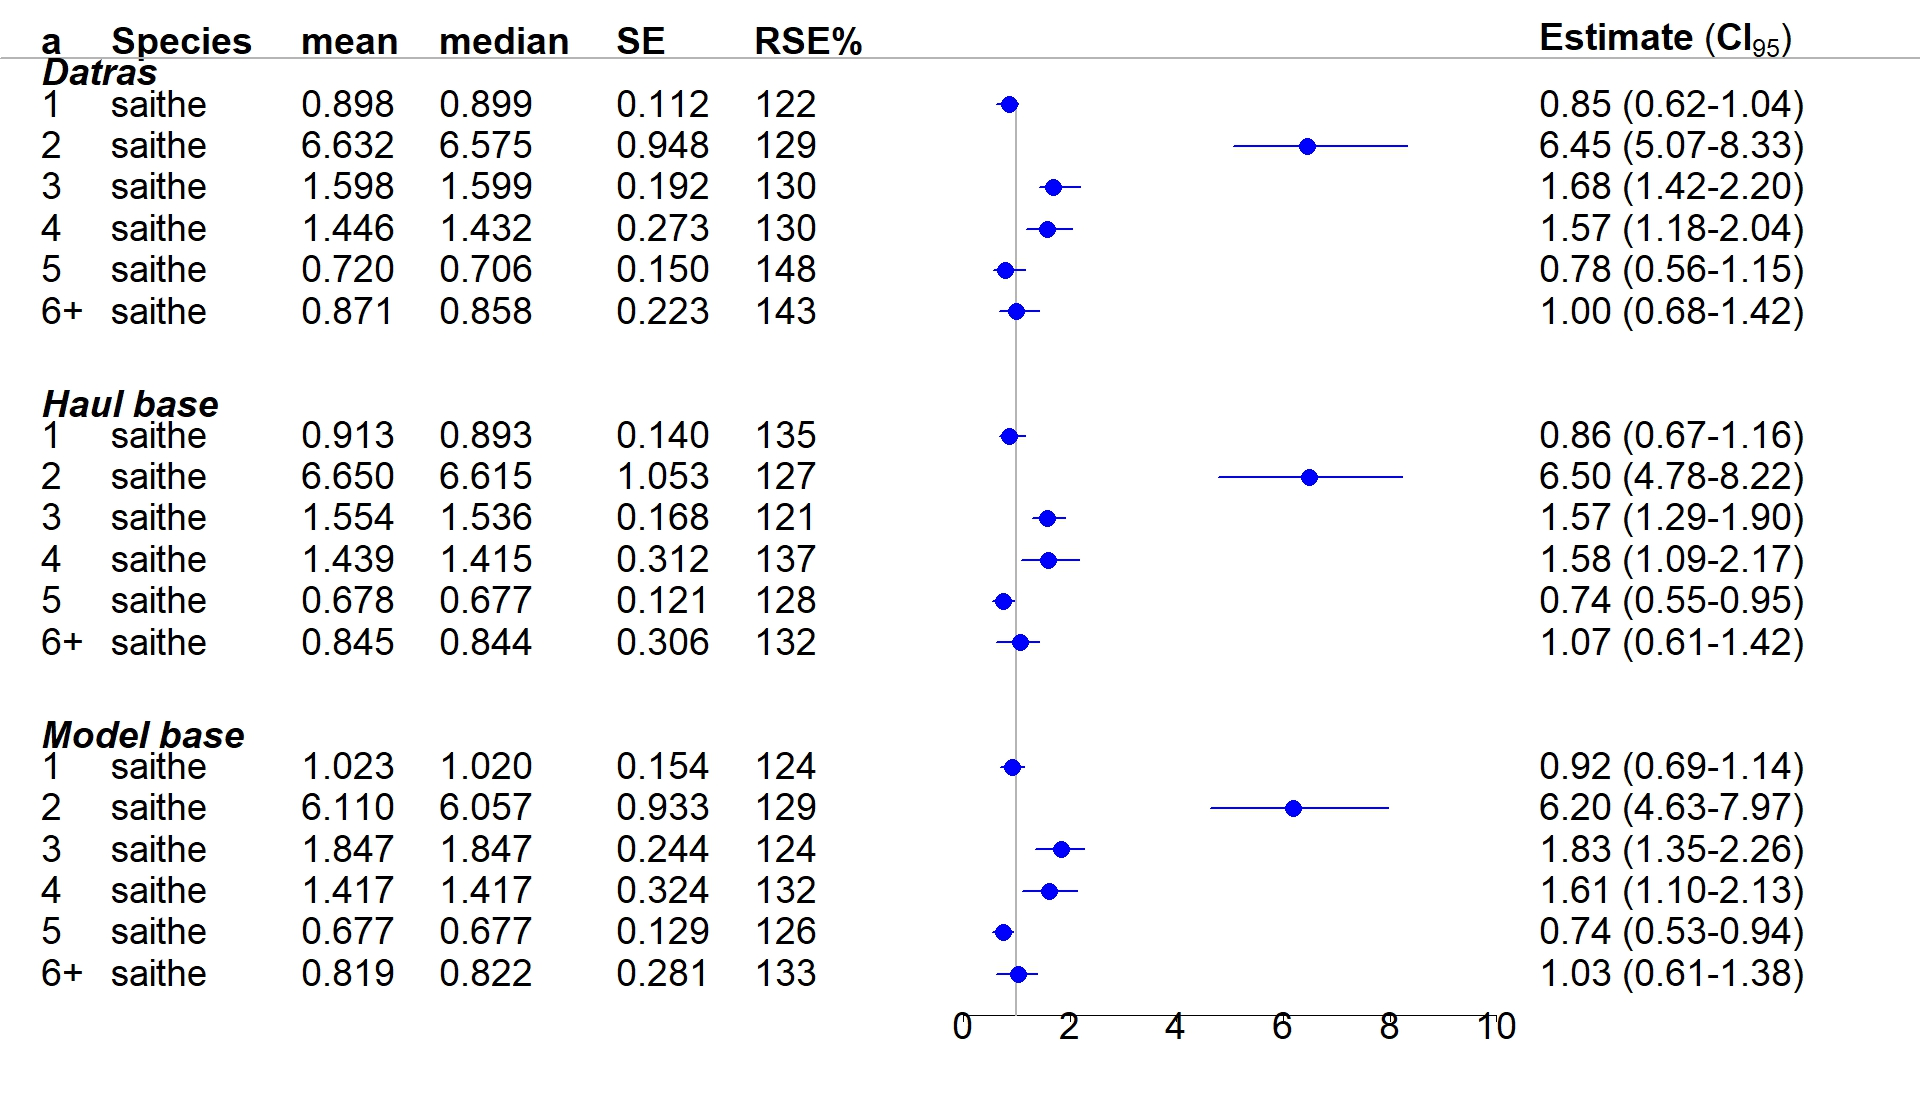
\includegraphics[width=0.95\textwidth]{saithe2018Q1BiasCorr.jpeg}} & \\
%\subfloat[Percentile bootstrap method]{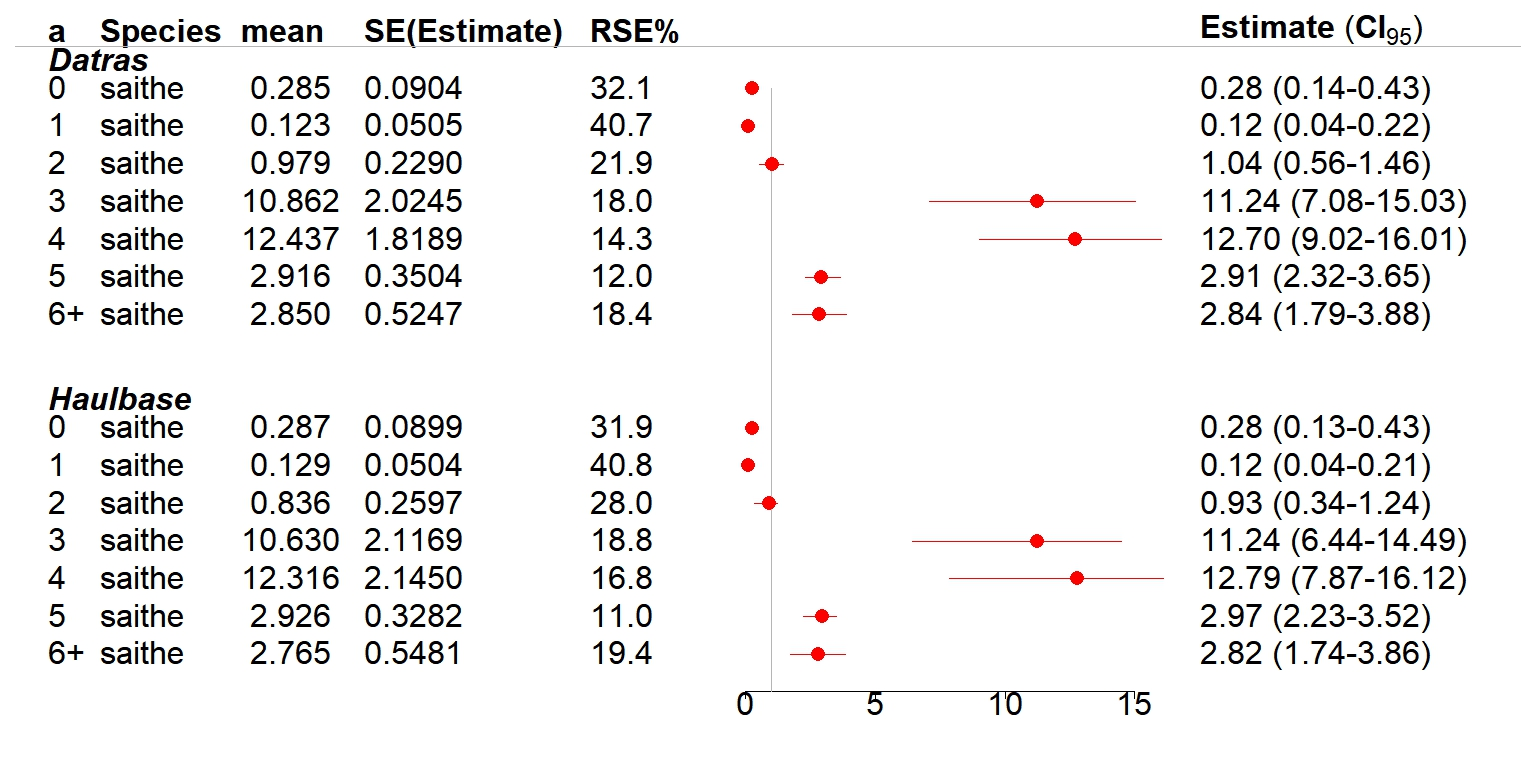
\includegraphics[width=0.95\textwidth]{saithe2017Q3Percentile.jpeg}} &
\end{tabular}
\caption[]{Estimated confidence intervals ($\mathrm{CI}_{96}$)  from bias-corrected bootstrap method for saithe in year 2018 Q1. Estimated indices of abundance (Estimate), and its standard error (SE), percentage relative standard error (RSE\%), bootstrap mean (mean) and median estimates are also given.}
\label{percentileBiascorrectedCIsaithe}
\end{figure*} 

%
%\clearpage
%\begin{itemize}
%
%\item \emph{more data in Q3 particularly for larger older fishes compared with Q1 hence overestimation due to ignoring of fine-scale stratification rather than fewer samples, hence higher variance; 48\% and 164\% increases for cod and saithe, respectively?}
%
%\item \emph{For all ALK methods the stratified bootstrap procedure is employed to estimate the uncertainty around indices of abundance. {\bf The estimated indices of abundance of cod are similar for all ALKs, but the the spatial ALKs generally gave higher estimates. Also, the spatial ALKs provide a better fit to the data in terms of precision. Uncertainty estimates (RSE) for older fishes ($\ge 4$) are higher, as expected, for the spatial ALKs as fewer samples are generally collected for these, and given that spatial variation in the data is accounted for, variability would be higher.}}
%
%\item \emph{generate plots for year 2018 Q1 cod and 2017 Q3 saithe. Possibly show same age given length group for both species? change plots to our show information in them- see the structure directly from the raw data that they correspond to the colours in the figure; TMB has problems when few observations are available-issues with the joint covariance matrix }
%\item have different plots...show fish of different ages (contours) corresponds to raw data, include points on the map of the different ages
%\item \emph{discuss differences in estimates from ALK methods (Table \ref{resultstablecodandsaithe} - in terms of relative standard error estimates; overestimation and underestimation from DATRAS (bootstrap) method not knowing the strength in either direction) - Issues:}
%\begin{itemize}
%\item \emph{Ignores fine scale stratification at the first stage, hence overestimation of the uncertainty}
%\item \emph{Ignores age-length data collected at the haul level, hence underestimates the uncertainty}
%\item \emph{Biases in both direction}
%\end{itemize}
%\item \emph{test for significant differences between estimates from ALK methods for age groups?}
%\item \emph{As discussed in Section \ref{sec:datrasalkestimator} and shown in the results in Table \ref{resultstablecodandsaithe} the assumption of no difference in regional compositions of age-length structures is invalid and DATRAS ALK have introduced bias in both direction, and the extent of this  bias in either direction is unknown. Hence, this ALK is not appropriate to perform further analyses. }
%\item \emph{codes do not run for saithe Q1 2018}
%\item \emph{Saithe and haddock tend to have a northerly distribution. The abundance of fish predators is generally lower in the German bight area. Within the northern area, saithe is more abundant in the eastern areas.}
%\item \emph{IBTS Q1 doesn’t cover the distribution of saithe adequately. Saithe are found deeper than the survey extends and any fluctuations in abundance within the survey are not related to stock size, but due to movement up and down the slope at that time. Explanation is in the 2016 benchmark report for saithe, available on the ICES website}
%\item \emph{The saithe assessment went through an ICES benchmark process in 2016 (ICES, 2016b). The scientific survey used in the assessment does not cover the whole stock distribution; however, it is considered generally representative. The number of observations (trawl stations) with saithe is low and the resulting survey index is uncertain. Commercial catch per unit effort information for French, German, and Norwegian trawlers was combined into a single index of biomass of fishable saithe. There are conflicting signals between the survey and fishable biomass index. The fraction of age 3 saithe migrating into the survey area (and the fishery) is low and varying between years with no obvious trend. Observations of saithe at age 3 are not suitable for predicting year-class strength. This means that assumed recruitment values are highly uncertain and a substantial portion $(30 \%)$ of the advised wanted catch in 2017 is based on the recruitment assumptions for 2016 and 2017 \citep{ICESJune2016}} 
%\end{itemize}


\clearpage
\subsection{Optimum sampling effort for North Sea Cod and Saithe}
\label{sec:optimumeffortresults}
In order to determine optimum sampling levels of otoliths for saithe and cod in the North Sea, ALKs are estimated using the haul based  method. As shown in Figures \ref{percentileBiascorrectedCIcod} and \ref{percentileBiascorrectedCIsaithe} the haul base ALK and the model base ALK gave similar estimates of abundance indices and precision as both approaches are attempting to account for spatial variation in the data. But, the spatial ALK model is  quite complex, and model fitting would be computer-intensive since the model must be fitted for each bootstrap run and each simulated sampling procedure that mimics the real data collection procedure. For this reason, the model base ALK approach will not be used in this analysis. Also, the assumption of no difference in regional compositions of age-length structures is invalid,  as shown in Figure \ref{predictedprobabilitiesplot},  so DATRAS ALK is not use for further analyses. The removal procedure for otolith sampling described in Section \ref{sec:optimizationsampling} is applied to data in year 2018 Q1 for cod and year 2017 Q3 for saithe.

%\begin{itemize}
%\item \emph{We can include a similar plot with 2017 (saithe) and 2018 (cod) data  here to show that it's reasonable to group at 2cm and 5 cm? Explain why 2 cm or 5 cm is chosen as illustrations?}
%\item \emph{include (cm) on the x-axis to demonstrate the unit used for length; write out the word "probability" on y- axis; remove bold titles on the plots; show real data plot alongside these plots}
%\end{itemize}
%
%\clearpage
%
%\begin{figure*}[h!]
%\centering
%\begin{tabular}{@{}ccc@{}}
%\subfloat[age-length distribution of cod]{\includegraphics[width=0.45\textwidth]{cod2018Q1StatRec43F6.jpeg}} & 
%\subfloat[age-length distribution of saithe]{\includegraphics[width=0.45\textwidth]{cod2018Q1StatRec47E8.jpeg}} &
%\end{tabular}
%\caption[]{Predicted probabilities of age given length using the model described in (\ref{eq:linearPred1}) and (\ref{eq:linearPred}) for cod (left panel) and saithe (right panel) in Q1 and Q3, respectively in year 2015.}
%\label{fig:agelengthplot}
%\end{figure*} 
%For each sampling procedure, the number of otoliths removed for cod is 


In year 2018 Q1, the number of otoliths sampled for cod was 1511, of which .........were removed in the experiments 1 cm, 2 cm, 3 cm, 4 cm, 5 cm or 7 cm length group, respectively. In year 2017 Q3, 2092 otoliths were sampled for saithe and ........were removed in the experiments 1 cm, 2 cm, 3 cm, 4 cm, 5 cm or 7 cm length group, respectively. Figure\ref{reduceresults} gives estimates of abundance for the original data, estimated indices for the reduced data, and their standard errors, and approximate 95\% confidence intervals for  $200$ simulations and $200$ bootstrap replication. 

The effect on abundance indices for 3 cm length or less is minimal for all age groups ............. 

\clearpage
Note that the nonparametric bootstrap method is advantageous  because it does not assume any distribution for the data, and it also accounts for some of the variability in the sampling distribution of the CPUE, however, there are some limitations of this method. The most important limitation is the assumption that the distribution of the data represented by the sample is a reasonable estimate of the population function from which the data are sampled. If this assumption is violated the random sampling  performed in the bootstrap procedure may add another level of sampling error, resulting in invalid statistical estimations \citep{haukoos2005advanced}. As discussed in Section \ref{overview} the selection of the trawling locations in IBTS is semi-random where cruise leaders selects "clear" tow locations or "blind" tow locations if no clear tow exists by checking the proposed trawl track for hazardous seabed obstructions with acoustic methods. More recently selection of tow locations is based on pre-proposed valid tow locations with start and end positions executed in the period 2000-2017. Hence, the lack of a fully randomized sampling process has the potential to result in biased estimates of parameters and their uncertainty. Random sampling performed in the bootstrap procedure also adds another level of potential sampling error, which is reflected in variation and biased estimates commonly performed in the bootstrap analysis. Note that the sampling distribution of the bootstrapped statistics is frequently not symmetric and computing point estimates from in this manner may reflect biased estimation from the samples. This can be seen in the estimated bootstrap mean values in Figure \ref{reduceresults}


\clearpage

\begin{figure*}[h!]
\centering
\begin{tabular}{@{}ccc@{}}
\subfloat[Cod in year 2018 Q1]{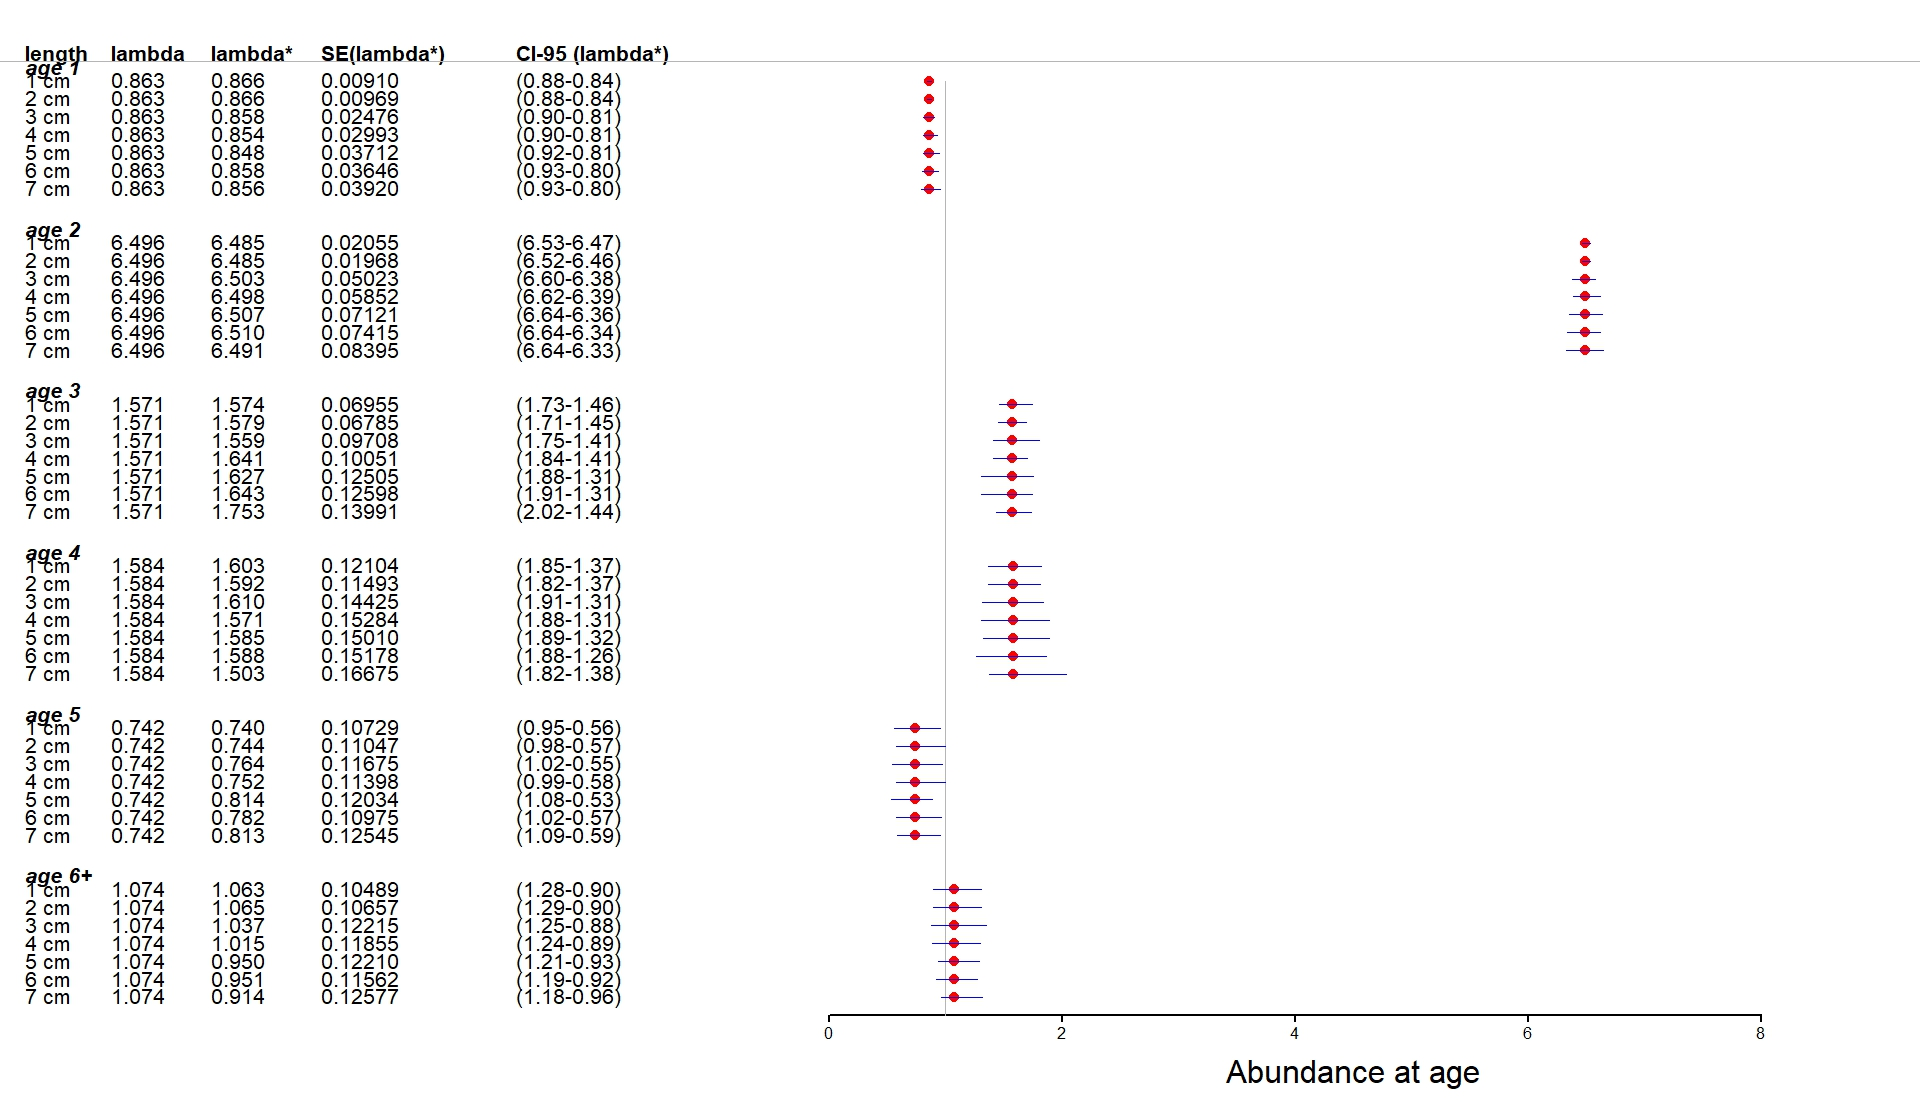
\includegraphics[width=1.05\textwidth]{cod2018Q1ReducedData.jpeg}} & \\
\subfloat[Saithe in year 2017 Q3]{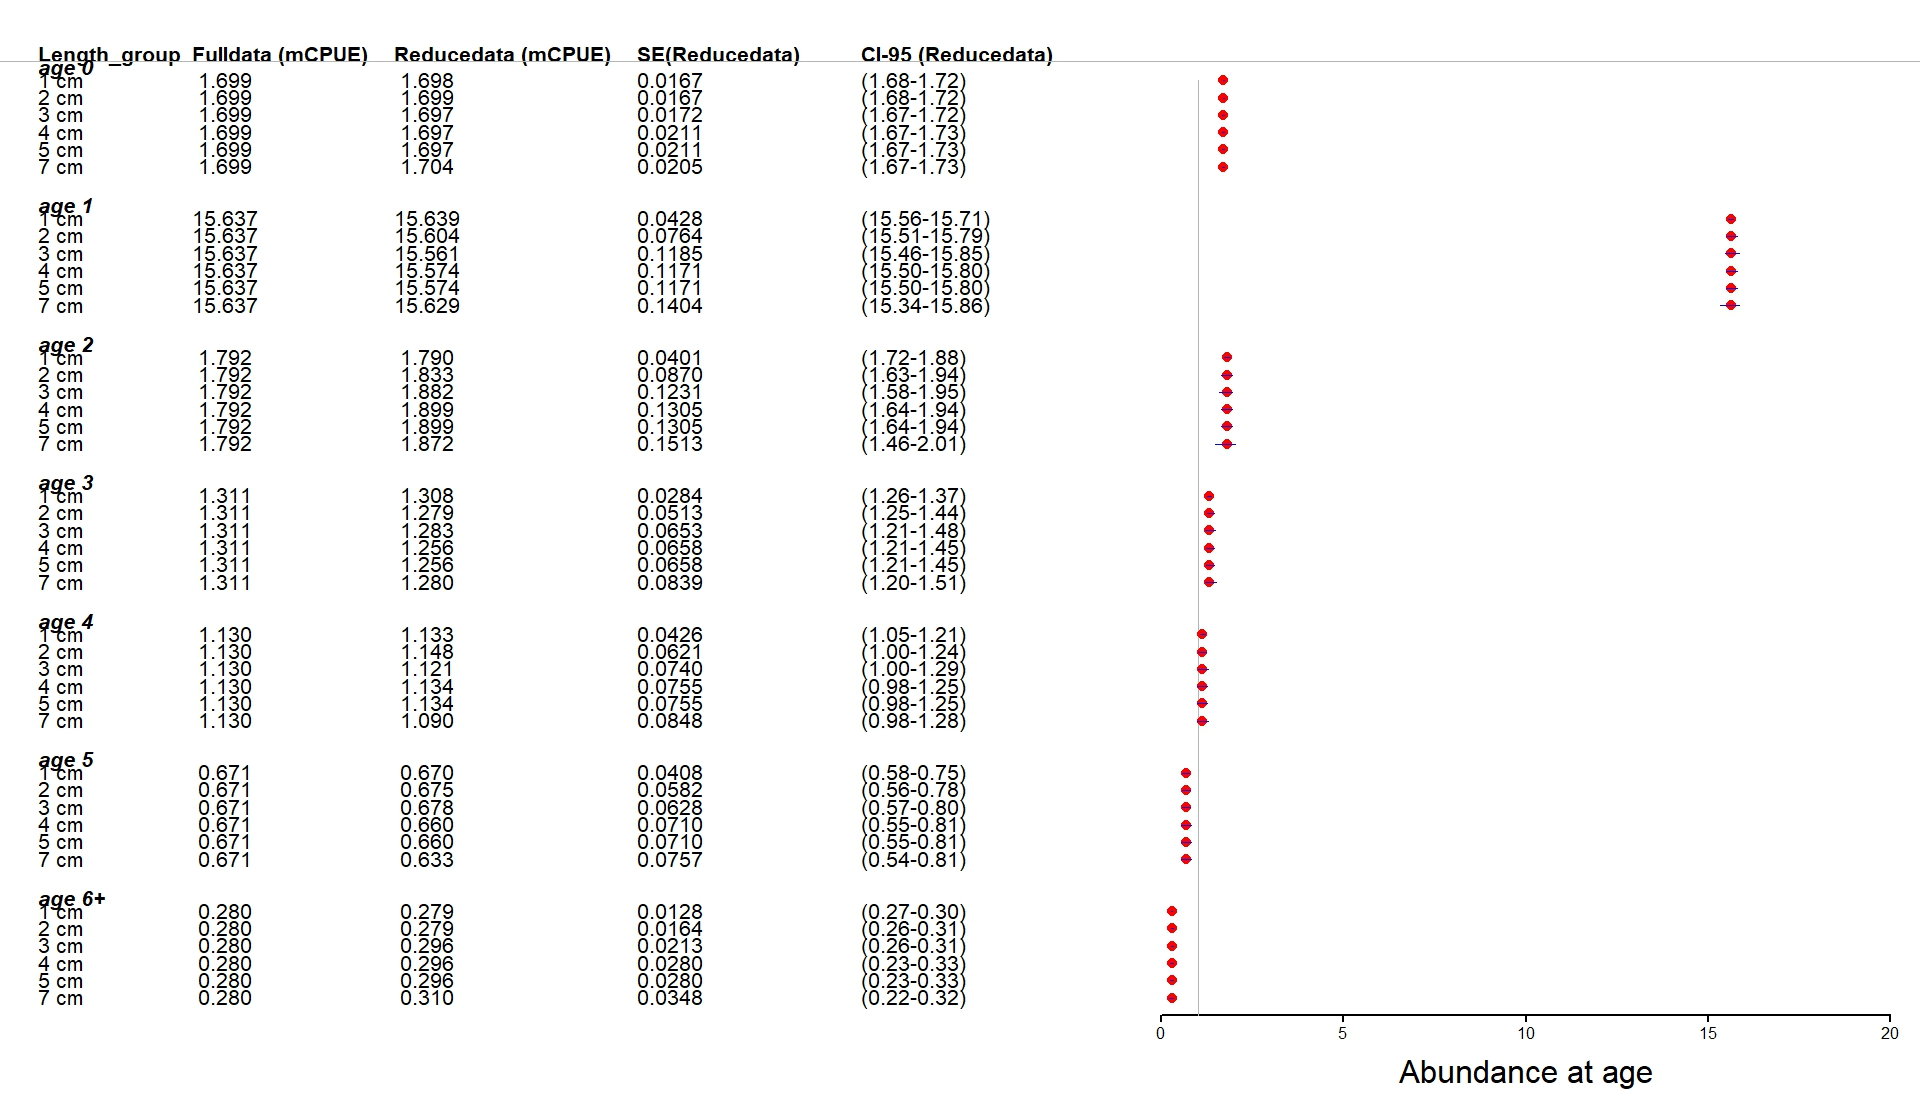
\includegraphics[width=1.05\textwidth]{saithe2017Q3ReducedData.jpeg}} &
\end{tabular}
\caption[]{Comparing estimated abundance from the original data where one otolith per length group: 1cm, 2cm, 3cm, 4cm, 5cm or 7cm is sampled for cod in year 2018 Q1 and saithe in year 2017 Q3. Estimated confidence intervals ($\mathrm{CI-95}$), and its standard error (SE) estimates of the reduced samples are also given.}
\label{reduceresults}
\end{figure*} 

%
%\clearpage
%\begin{figure*}[h!]
%\centering
%\begin{tabular}{@{}ccc@{}}
%\subfloat[Saithe in year 2017 Q3]{\includegraphics[width=1.05\textwidth]{cod2017Q3ReducedData.jpeg}} & \\
%%\subfloat[Cod in year 2017 Q3]{\includegraphics[width=1.05\textwidth]{cod2017Q3ReducedData.jpeg}} &
%\end{tabular}
%\caption[]{Comparing estimated abundance from the original data where one otolith per length group: 1cm, 2cm, 3cm, 4cm, 5cm or 7cm is sampled for cod  in year 2017 Q3. Estimated confidence intervals ($\mathrm{CI-95}$), and its standard error (SE) estimates of the reduced samples are also given.}
%\label{reduceresultscode2017}
%\end{figure*} 


%
%\begin{itemize}
%\item \emph{The time needed for estimating the model varies slighlty between species and year. A laptop with  processor intel(R) Core(TM) i5-6300 CPU @ 2,40 GHz, used e.g. approximately 2 minutes to estimate the parameters for cod in year 2018.}
%\item \emph{discuss effects of this reduction on estimate and variance}
%\item \emph{extract data for number or percentage of otoliths removed when 2 cm or 5 cm removal procedure is used and fill ${\bf x}$  and ${\bf y}$ in text with values }
%\item include no otoliths for each section ---all data, reduced data by 2 cm etc
%\end{itemize}

\clearpage

\section{DISCUSSION}
\label{sec:discussion}

In this research we have determined minimum sampling efforts of otoliths for target species of the North Sea International Bottom Trawl Survey. This was achieved by testing sampling procedures that mimic the real data collection procedure but with a reduced number of otoliths. Several sampling procedures were tested and the effect on estimated abundance indices and their variance were investigated. Abundance indices were estimated using age-length keys (ALKs). The database for trawl surveys (DATRAS) manned by ICES includes an ALK that uses the raw proportions of age given length assuming constant age-length compositions over relatively large areas. We have developed two spatial ALK methods  to estimate abundance indices and their variance that accounts for spatial variation in the data: 1) a haul based ALK that produces an ALK for each trawl haul, and which uses the raw proportions of age given length, and 2) a spatial ALK model that uses logits for modelling the age distribution in catch data from the length-stratified  subsamples. Several studies have used spatial ALK modelling for estimating abundance indices of the North Sea stocks used in  assessments \citep{berg2012spatial, berg2014evaluation, gerritsen2006simple}. These studies used continuous ratio logits with General Linear Model (GLM) or General Additive Models (GAMs) to model the spatial effects and found regional effects...... We propose to use Gaussian Random Field Theory to model the spatial effects as a smooth surface.........

\begin{itemize}
\item \emph{discuss positives of using GRT to model spatial effects: what problems are eliminated when using this in terms of missing data}
\item \emph{compare the effects of our method with GAMs \citep{berg2012spatial} and \citep{berg2014evaluation} and the NS-IBTS Delta-GAM index for estimating standardized age-based indices and the species theses are used for to include in assessment}
\item \emph{what does our model allows in terms of the age groups (samller or higher age groups (6+) possible with our model); covariates such as haul effect (included as a random effect)}
\end{itemize}

Also, both spatial ALK methods proposed in this paper provided a much better fit to the data compared with DATRAS ALK....

Reducing the number of otoliths by ${\bf x}$ percent had {\bf no} significant effect on estimated abundance
\begin{itemize}
\item \emph{discuss sampling procedure: limitation and advantages; and possibly more advanced selection procedures? }
\item \emph{new approach adopted in surveys from 2018 }
\item \emph{IBTS has a standardized survey indices? -(yes Berg's NS-IBTS Delta-GAM index).  so changes in catch rates are due to changes in population size? \citet{berg2014evaluation} developed a standardized index for IBTS data but only applied to some species e.g., haddock? cod- last year 2017. Is the designed based age index on DATRAS not a standardized index?}
\item \emph{how does changes in survey design or other factors affect changes in catch rates? If so are these changes  significant? }
\end{itemize}


\section{General comments}

\begin{itemize}
\item Decide on whether we say, "in this research or paper"
\item Decide on whether to say, "In this subsection or section"
\item Decide on year of data for case studies
\item Decide on writing "haul(model)-based or haul (model) based
\item Decide on calling the survey "The North Sea IBTS or IBTS"
\item Decide on writing "Cod or cod, and Saithe or saithe"
\item Decide on a title for the paper
\item {\bf what are issues with including haul effect in model based ALK?
 (Olav)}
 
\end{itemize}

\clearpage








\clearpage

\bibliographystyle{apalike}
\bibliography{ibtsBib}

\clearpage

\appendix


\clearpage
\section{\large Areas fished by different countries in the North Sea IBTS}
\label{secAp:areasfishedappendix}
Typically, two different countries fish each rectangle so that at least two trawl hauls are made per rectangle, but intensified sampling is carried out in the following areas: at least 3 hauls per rectangle are taken in statistical rectangles  31F1, 31F2, 32F1, 33F4, 34F2, 34F3, 34F4, 35F3, 35F4; while six or more hauls per rectangle are taken in statistical rectangles  30F1, 32F2, 32F3, 33F2, 33F3 (ICES 1999).  The Skagerrak and Kattegat is fished solely by Sweden, who sample more than once in every rectangle while the west of Shetland (in Q1 and Q3) and inshore areas (Q3) is fished solely by Scotland. The edge of the Norwegian Trench is fished solely by Norway, but inshore areas near Denmark is fished by Denmark. The southern North Sea is fished by Denmark, Germany and England. France, typically, is the only country that surveys the western English Channel. Areas are surveyed by a single country because of the large proportion of untrawalable area (and subsequent gear damage issues experienced by other nations)  for efficient logistical purposes. Table \ref{countries} gives the countries and research vessels participating the North Sea IBTS.\\
\begin{small}
\begin{table}[h!]
\centering
\captionsetup{font=small, width = 15.5cm}{
\caption{Survey countries, vessel name, and period research vessels participating in first quarter (Q1) and third quarter (Q3) during 1997-2017.}\label{countries}}
\begin{tabular}{cccccccc}
\hline \\[0.1ex]
  & \multicolumn{2}{c}{\bf First Quarter (Q1)} & \multicolumn{2}{c}{\bf Third Quarter (Q3)}\\[1.5ex]
{\bf Country }  & Vessel name & Period    & Vessel name & Period  \\[0.5ex]
\hline \\[0.5ex]
Denmark  &   Dana   &   January-February  & Dana & July-August    \\[1ex]
France  & Thalassa II & January-February & - & -   \\[1ex]
Germany   &  Walther  Herwig III & January-February   &   Walther  Herwig III & July-August \\[1ex]
Netherlands &  Tridens 2 &  January-February   & - & -     \\[1ex]
Norway  &   G.O. Sars  & January-February &    Johan Hjort  & July   \\[1ex]
UK England &- & -&  Endeavour &  August-September  \\[1ex]
UK Scotland   &  Scotia III &  January-February & Scotia III &  July-August \\[1ex]
Sweden  &  Dana &  January-February  &  Dana &  August                  \\[0.5ex]
\hline
\end{tabular}
\end{table}
\end{small}

\section{\large Otolith sampling per fish species}
\label{secAp:otolithappendix}
From 1991-2017, most countries conducted quota sampling of otoliths per length group in a RFA. But from 2013 Norway has been sampling one otolith per length class from each trawl haul (to 0.1$\cm$ below for shellfish, to 0.5$\cm$ below for herring and sprat and to 1$\cm$ below for all other species). From the first quarter in 2018 all countries are required to sample one otolith per length class per trawl haul.  Table \ref{tab:otolithsTable} gives the minimum sampling levels of otoliths for the target species. However, for the smallest size groups, that presumably contain only one age group, the number of otoliths per length class may be reduced, and more otoliths per length are required for the larger length classes. \\
%\clearpage
\begin{small}
\begin{table}[h!]
\centering
\caption{Minimum sampling levels of otoliths by species for RFA or per trawl haul.}
\label{tab:otolithsTable}
\begin{tabularx}{\linewidth}{r l l l l X}
\toprule 
Period &  Species  & Minimum sampling levels of otoliths per length class    \\[0.7ex]
\midrule \\[0.1ex]
{\bf 1991-2017} & & {\bf Number of otoliths per length class in a RFA}  \\[1.8ex]
     & herring  &  $8$  otoliths per $\frac{1}{2}$ cm group \\[0.8ex]
     & sprat    & $16$  otoliths per $\frac{1}{2}$ cm length class  $8.0 -11.0$ cm\\[0.8ex]
              & & $12$  otoliths per $\frac{1}{2}$ cm length class  $\geq 11.0$ cm\\[0.8ex]
& mackerel      & $8$  otoliths per $\frac{1}{2}$ cm length class \\[0.8ex]
& cod       	  & $8$  otoliths per $1$ cm length class\\[0.8ex]
&haddock   	  & $8$  otoliths per $1$ cm length class \\[0.8ex]
&whiting    	  & $8$  otoliths per $1$ cm length class \\[0.8ex]
&Norway pout   & $8$  otoliths per $1$ cm length class\\[0.8ex]
&saithe        & $8$  otoliths per $1$ cm length class \\[2ex] 
& All target species      &  From 2013 Norway and Scotland, and  Netherlands from 2016 \\[0.7ex] 
&& have been sampling 1 otolith per length class from each trawl haul \\[0.7ex] 
&& (to 0.1$\cm$ below for shellfish, to 0.5$\cm$ below for herring and sprat, and \\ [0.7ex] 
&& to 1$\cm$ below for all other species).\\[2.7ex] 

{\bf 2018} & & {\bf Number of otoliths per length class per trawl haul}  \\[1.8ex]
  & herring  &  $1$  otolith per $\frac{1}{2}$ cm group \\[0.8ex]
     & sprat    & $1$  otolith per $\frac{1}{2}$ cm length class  $8.0 -11.0$ cm\\[0.8ex]
              & & $1$  otolith per $\frac{1}{2}$ cm length class  $\geq 11.0$ cm\\[0.8ex]
& mackerel      & $1$  otolith per $1$ cm length class \\[0.8ex]
& cod       	  & $1$  otolith per $1$ cm length class\\[0.8ex]
& haddock & $2$  otoliths per $5$ cm length class $11 -15, \ 16-20, \ 21-25, \ 26-30$ cm \\[0.8ex]
& Norway pout & $2$  otoliths per $5$ cm length class $5 -10, \ 11-15$ cm\\[0.8ex]
               & & $2$  otoliths per $1$ cm length class $> 15$ cm\\[1.8ex]
&saithe        & $1$  otolith per $1$ cm length class \\[0.8ex]  
&plaice       & $1$  otolith per $1$ cm length class \\[0.5ex]
\bottomrule         
\end{tabularx}
\end{table}
\end{small}

%\clearpage
 \section{\large Weightings of Statistical Rectangles}
 \label{secAp:weightings}
%\clearpage 
 \begin{small}
\begin{table}[h!]
\centering
\caption{Weights used for Pollachius virens in equation (\ref{eq:cpueRec}).}
\begin{footnotesize}
\begin{tabular}{clclclclcl}
  \hline \\ [0.3ex]
 StatRec & Weight & StatRec & Weight & StatRec & Weight & StatRec & Weight & StatRec & Weight  \\ [1.0ex]
  \hline \\ [0.3ex]
 31F1 &  0.6 & 38F0 &    1 & 41F7 &    1 & 44F3 &    1 & 48E7 &    1 \\ 
 31F2 &  0.8 & 38F1 &    1 & 41F8 &  0.1 & 44F4 &    1 & 48E8 &  0.9 \\ 
 31F3 & 0.05 & 38F2 &    1 & 41G0 &  0.2 & 44F5 &  0.9 & 48E9 &    1 \\ 
 32F1 &  0.8 & 38F3 &    1 & 41G1 & 0.97 & 44F8 & 0.25 & 48F0 &    1 \\ 
 32F2 &    1 & 38F4 &    1 & 41G2 & 0.53 & 44F9 &  0.8 & 48F1 &    1 \\ 
 32F3 &  0.8 & 38F5 &    1 & 42E7 &  0.4 & 44G0 & 0.94 & 48F2 &    1 \\ 
 32F4 & 0.01 & 38F6 &    1 & 42E8 &    1 & 44G1 &  0.6 & 48F3 &  0.5 \\ 
 33F1 &  0.3 & 38F7 &    1 & 42E9 &    1 & 45E6 &  0.4 & 48G0 & 0.02 \\ 
 33F2 &    1 & 38F8 &  0.3 & 42F0 &    1 & 45E7 &    1 & 49E6 &  0.8 \\ 
 33F3 &    1 & 39E8 &  0.5 & 42F1 &    1 & 45E8 &    1 & 49E7 &    1 \\ 
 33F4 &  0.4 & 39E9 &    1 & 42F2 &    1 & 45E9 &    1 & 49E8 &  0.4 \\ 
 34F1 &  0.4 & 39F0 &    1 & 42F3 &    1 & 45F0 &    1 & 49E9 &    1 \\ 
 34F2 &    1 & 39F1 &    1 & 42F4 &    1 & 45F1 &    1 & 49F0 &    1 \\ 
 34F3 &    1 & 39F2 &    1 & 42F5 &    1 & 45F2 &    1 & 49F1 &    1 \\ 
 34F4 &  0.6 & 39F3 &    1 & 42F6 &    1 & 45F3 &    1 & 49F2 &    1 \\ 
 35F0 &  0.8 & 39F4 &    1 & 42F7 &    1 & 45F4 &  0.6 & 49F3 &  0.5 \\ 
 35F1 &    1 & 39F5 &    1 & 42F8 &  0.2 & 45F8 &  0.3 & 50E6 &  0.1 \\ 
 35F2 &    1 & 39F6 &    1 & 42G0 & 0.32 & 45F9 & 0.02 & 50E7 &  0.6 \\ 
 35F3 &    1 & 39F7 &    1 & 42G1 & 0.89 & 45G0 & 0.24 & 50E8 &  0.7 \\ 
 35F4 &  0.9 & 39F8 &  0.4 & 42G2 & 0.64 & 45G1 & 0.55 & 50E9 &  0.9 \\ 
 35F5 &  0.1 & 40E7 & 0.04 & 43E7 & 0.03 & 46E6 &  0.4 & 50F0 &    1 \\ 
 36F0 &  0.9 & 40E8 &  0.8 & 43E8 &  0.9 & 46E7 &  0.9 & 50F1 &    1 \\ 
 36F1 &    1 & 40E9 &    1 & 43E9 &    1 & 46E8 &    1 & 50F2 &    1 \\ 
 36F2 &    1 & 40F0 &    1 & 43F0 &    1 & 46E9 &    1 & 50F3 &  0.2 \\ 
 36F3 &    1 & 40F1 &    1 & 43F1 &    1 & 46F0 &    1 & 51E6 &    0 \\ 
 36F4 &    1 & 40F2 &    1 & 43F2 &    1 & 46F1 &    1 & 51E7 &    0 \\ 
 36F5 &    1 & 40F3 &    1 & 43F3 &    1 & 46F2 &    1 & 51E8 &  0.5 \\ 
 36F6 &  0.9 & 40F4 &    1 & 43F4 &    1 & 46F3 &  0.8 & 51E9 &    1 \\ 
 36F7 &  0.4 & 40F5 &    1 & 43F5 &    1 & 46F9 &  0.3 & 51F0 &    1 \\ 
 36F8 &  0.5 & 40F6 &    1 & 43F6 &    1 & 46G0 & 0.52 & 51F1 &    1 \\ 
 37E9 &  0.2 & 40F7 &    1 & 43F7 &    1 & 46G1 &  0.2 & 51F2 &  0.5 \\ 
 37F0 &    1 & 40F8 &  0.1 & 43F8 & 0.94 & 47E6 &  0.8 & 51F3 &    0 \\ 
 37F1 &    1 & 41E6 & 0.03 & 43F9 & 0.41 & 47E7 &  0.6 & 52E6 &    0 \\ 
 37F2 &    1 & 41E7 &  0.8 & 43G0 & 0.21 & 47E8 &    1 & 52E7 &    0 \\ 
 37F3 &    1 & 41E8 &    1 & 43G1 &  0.7 & 47E9 &    1 & 52E8 &    0 \\ 
 37F4 &    1 & 41E9 &    1 & 43G2 &  0.3 & 47F0 &    1 & 52E9 &  0.1 \\ 
 37F5 &    1 & 41F0 &    1 & 44E6 &  0.5 & 47F1 &    1 & 52F0 &  0.2 \\ 
 37F6 &    1 & 41F1 &    1 & 44E7 &  0.5 & 47F2 &    1 & 52F1 &  0.5 \\ 
 37F7 &    1 & 41F2 &    1 & 44E8 &  0.9 & 47F3 &  0.6 & 52F2 &  0.1 \\ 
 37F8 &  0.8 & 41F3 &    1 & 44E9 &    1 & 47F9 & 0.01 &  &  \\ 
 38E8 &  0.2 & 41F4 &    1 & 44F0 &    1 & 47G0 &  0.3 &  &  \\ 
 38E9 &  0.9 & 41F5 &    1 & 44F1 &    1 & 47G1 & 0.02 &  &  \\ 
 52F3 &    0 & 41F6 &    1 & 44F2 &    1 & 48E6 &    1 &  &  \\ 
   \hline \\[0.8ex]
\end{tabular}
\label{tab:weights}
\end{footnotesize}
\end{table}
 \end{small}
 
% \clearpage
\section{\large Imputation for missing age samples}
\label{sec:imputationappendix}
Catches of the target species are sampled (or subsampled with a size of 100 if the catches are too large) for length, and otoliths are typically collected from a subsample of the individuals sampled for length in the RFA,  or per trawl haul as in the case of Norway for determining age of the fish (see Table \ref{otolithsTable}). In the case of Norway where all trawl hauls are sampled for otoliths, missing age samples would still occur for the following two reasons: 1) the fish is below minimum length for otolith sampling (unreadable otoliths) or 2) otoliths are misplaced. Abundance indices by age group are estimated based on three age-length-keys (ALK): 1) DATRAS ALK estimator, 2) Haul dependent ALK estimator, and 3) Spatial model-based ALK estimator.
\subsection{\normalsize DATRAS ALK Borrowing Approach}
\label{secAp:DATRASBorrow}
The ALK proposed in DATRAS (ICES 2013), which is an aggregation of individual samples from a haul combined over a round fish area (RFA), and missing age samples are imputed as follows: 
\begin{enumerate}
\item If there is no ALK for a length in the CPUE dataframe, age information is obtained accordingly
\begin{itemize}
\item If length class (CPUE) $<$ minimum length class (ALK), then age=1 for the first quarter and age=0 for all other quarters
\item  If minimum length class (ALK) $<$ length class (CPUE) $<$ maximum length (ALK) then age is set to the nearest ALK. If the ALK file contains values at equal distance, a mean is taken from both values. 
\end{itemize}
\item If length class (CPUE) $>$ maximum length (ALK) age is set to the plus group.
\end{enumerate}
The underlying assumption of this ALK approach is that age-length compositions are homogeneous within the superstrata. 
\subsection{\normalsize Haul-based ALK Borrowing Approach}
\label{secAp:oursBorrow}
\indent  The second is an a haul dependent ALK estimator which we propose, and is denoted by $\mathrm{ALK}^{H}$. Since the age-length composition of fish may be space-variant, that is, there may be variation in age-length compositions between trawl stations within a superstrata, the spatial dependence of the age-length composition must be accounted for to produce reliable estimates of the CPUE per age estimates. If this spatial dependence is ignored not only will estimates of abundance be biased but the impact on the variance may be substantial. So for each trawl haul an $\mathrm{ALK}^{H}$ is produced. \emph{Since there are few or none observations of ages for each length class in a trawl haul, length classes are therefore pooled in increasing order such that there are five length classes in each pooled length group. To replace missing values for the age distribution in the pooled length groups the method of "borrowing" ages from length groups in trawl hauls closest in air distance within the RFA is used. If there are no observed ages in the pooled length group in the RFA, missing values for the age distribution are replaced following the procedure outlined in the DATRAS ALK procedure (\ref{secAp:DATRASBorrow}) in step 1.  }

\section{\large Estimates from DATRAS and Stratified bootstrap procedures}
\label{secAp:resultsdatrasALK}
The naive bootstrap procedure prosed by DATRAS lacks the potential to account for the spatial variation in the data. The DATRAS bootstrap procedure ignores the fine-scale stratification in the sampling process, leading to an overestimation of the uncertainty; and ignores the age-length data collected at the haul level, resulting in an underestiamtion of the uncertainty. The results (Table \ref{percentileBiascorrectedCIProcedures}) shows an overestimation of the uncertainty for all age groups, suggesting that it is relevant to account for the fine-scale stratification when resampling the data.


\begin{figure*}[h!]
\centering
\begin{tabular}{@{}ccc@{}}
\subfloat[Datras and Stratified bootstrap Procedures]{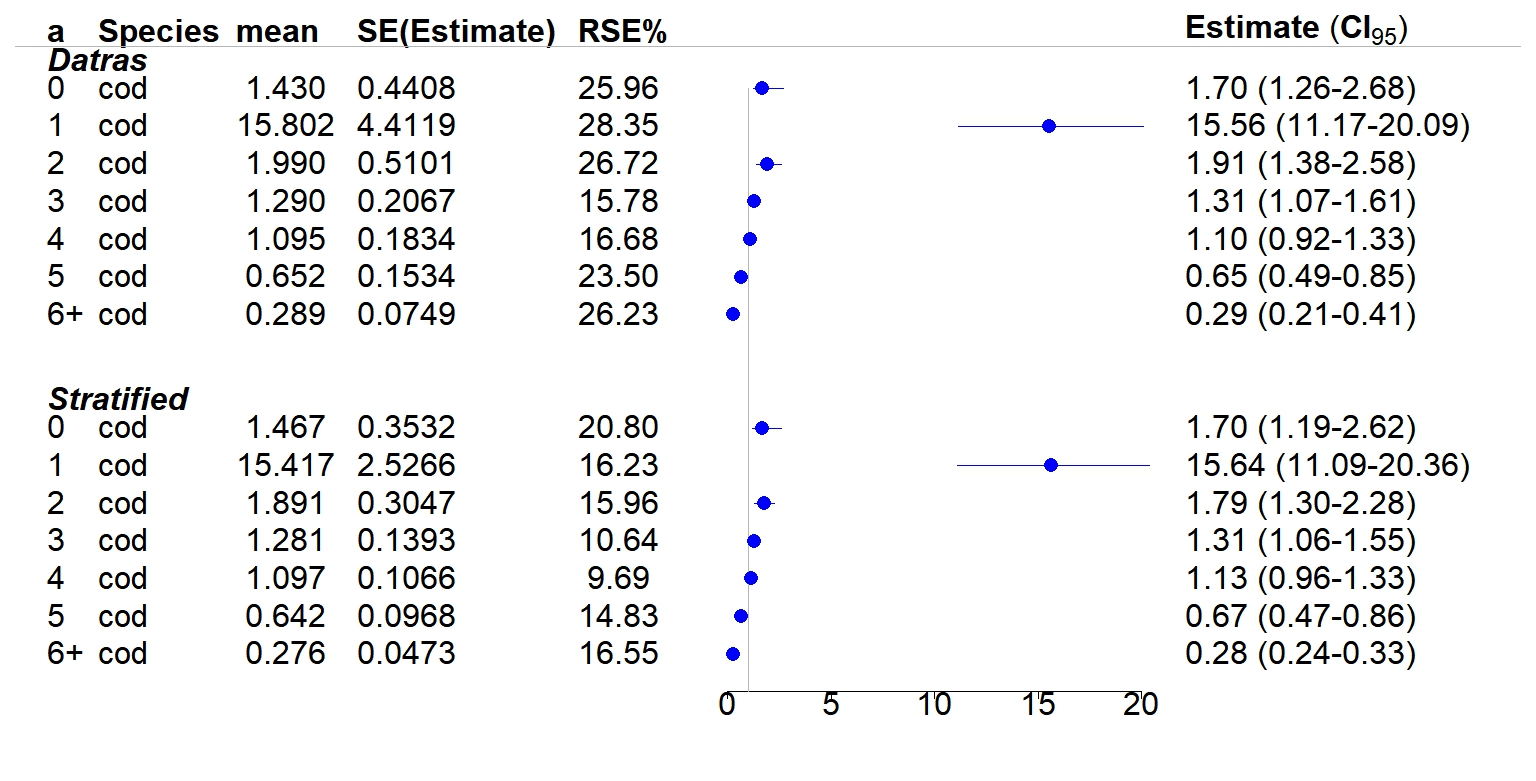
\includegraphics[width=0.95\textwidth]{cod2017Q3BootstrapProcedures.jpeg}} & 
\end{tabular}
\caption[]{Comparison of estimated confidence intervals ($\mathrm{CI}_{96}$) from Datras and stratified bootstrap procedures. The bias-corrected bootstrap method is used to give estimates for cod in year 2017 Q3. Estimated indices of abundance (Estimate), and its standard error (SE(Estimate), bootstrap mean (mean) and median estimates are also given.}
\label{percentileBiascorrectedCIProcedures}
\end{figure*} 




%\end{appendices}

\end{document}